\section{Eläinten joulu Meriharjussa}

\textit{Gustaf Björkenheimin rakennuttama Villa Meriharju on vuonna 1910 
valmistunut huvila Uutelassa. Nykyään huvila on Helsingin kaupungin 
omistuksessa ja se kulkee nimellä Meriharjun luontotalo. Rusakot ovat tehneet 
pikkujouluretkiä luontotalolle jo useamman kerran, vuosina 1996--2001, 2003, 
2008, 2009, 2015, 2016 ja 2019--2023. Myös vuoden 2024 pikkujouluretki 
suuntautui Meriharjuun -- lue lisää retken tapahtumista tästä jutusta!}

\begin{figure}[!b]
\centering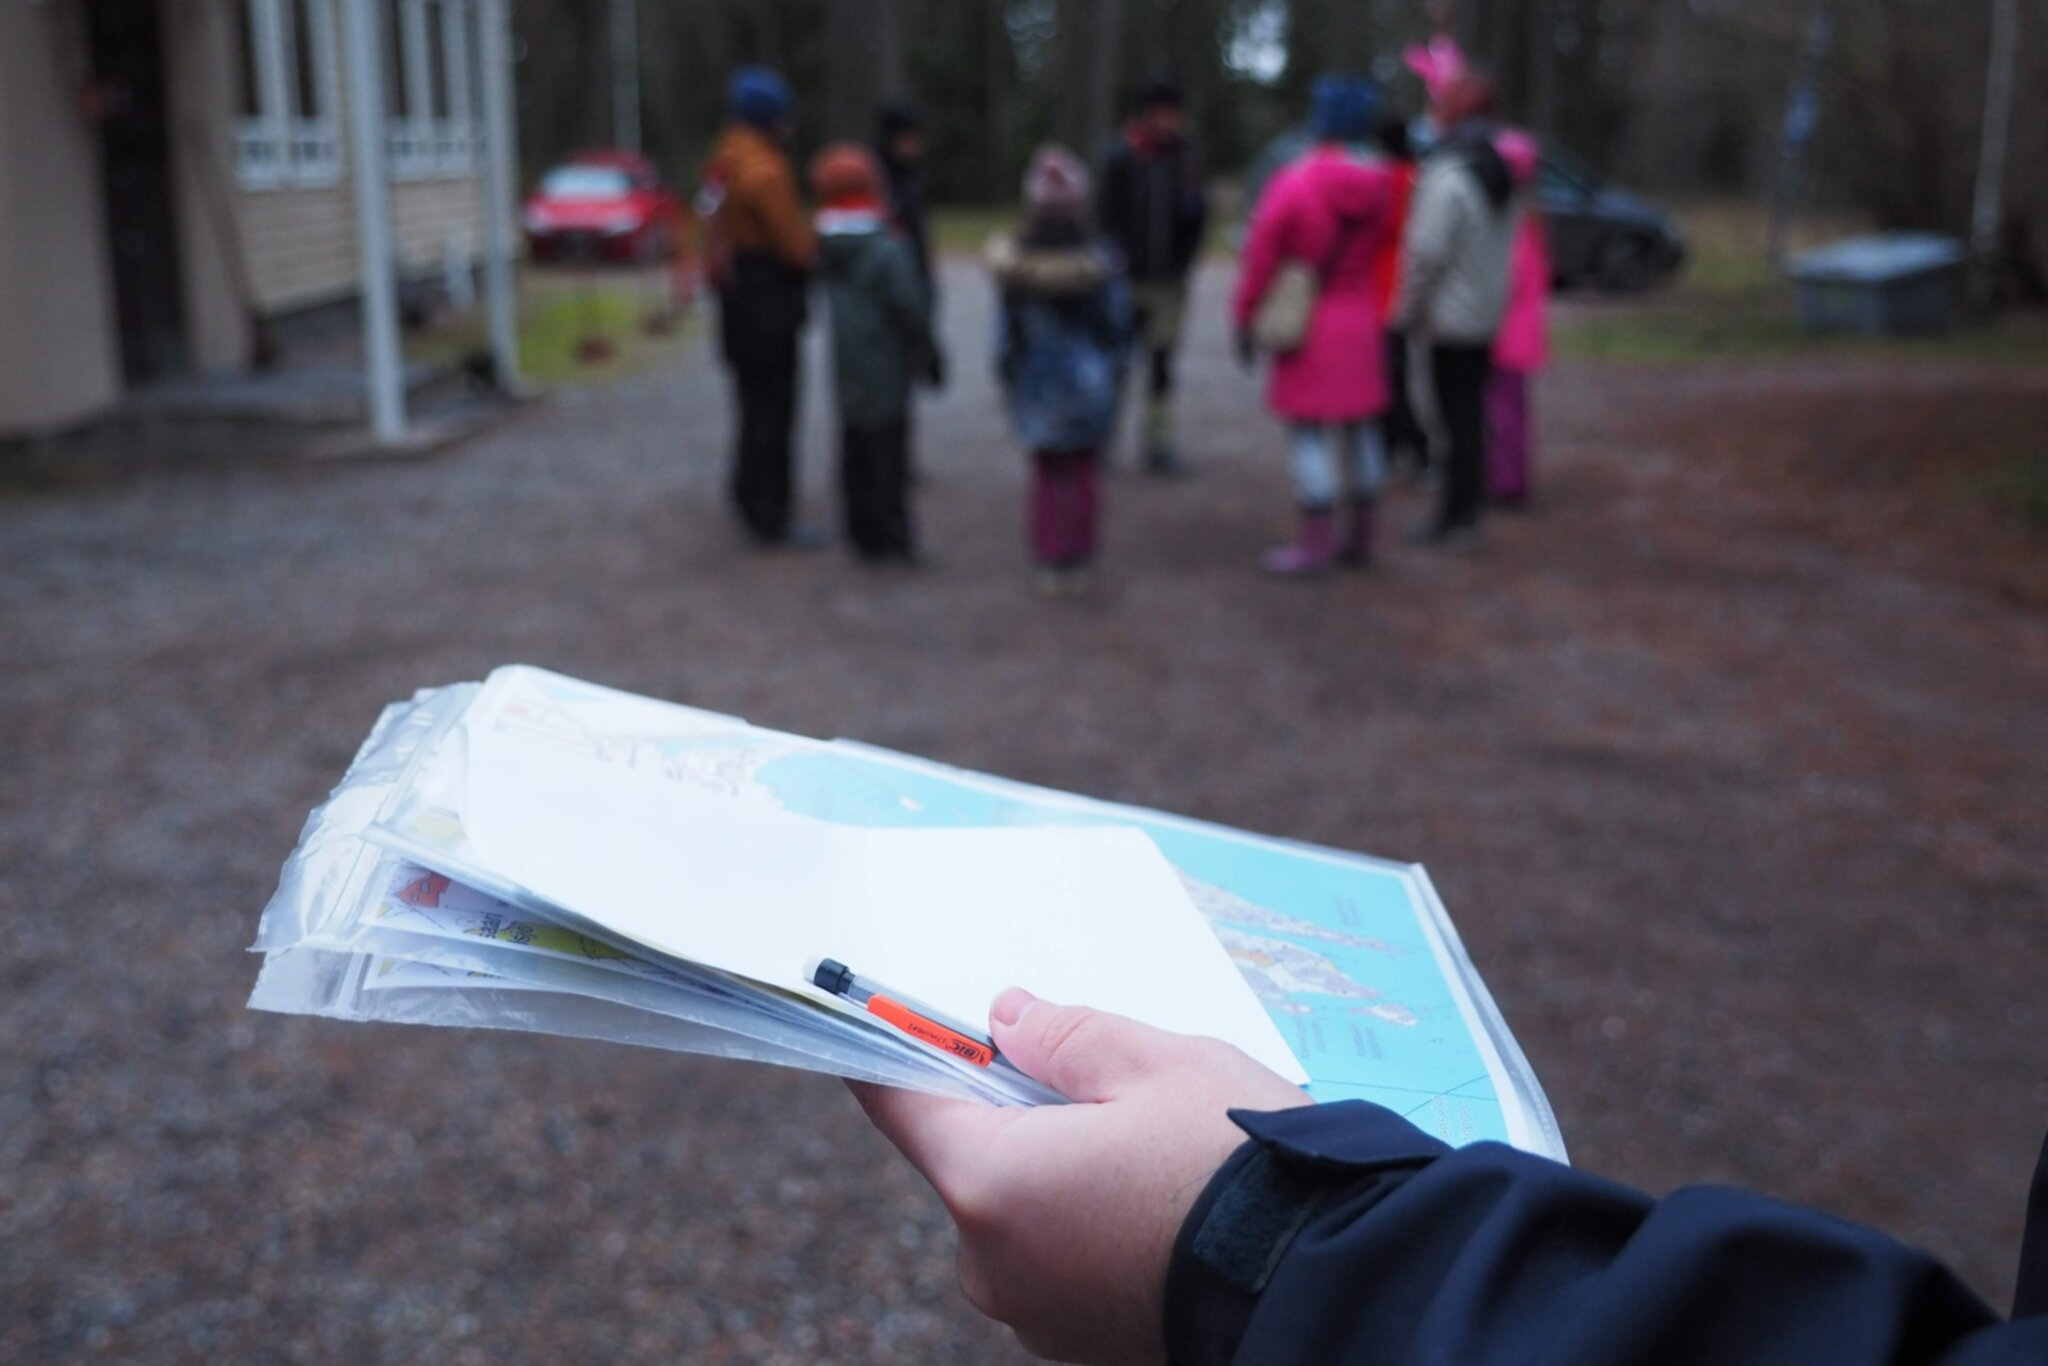
\includegraphics[width=\textwidth]{assets/meriharjuSuunnistus}
\caption{Lippukuntaretken lauantaisuunnistus käynnistyi luontotalon edustalta.}
\end{figure}

\begin{multicols}{2}
\noindent Kautta aikain rusakoiden pikkujouluretkillä on ollut erilaisia 
teemoja. Viime vuosina teemoina ovat olleet Itämeri, lentokykynsä 
menettäneet joulupukin porot, Kalevalan joulu sekä karanneet ja vilustuneet 
lehmät. Rusakoiden Meriharjun 17. pikkujouluretken teemana oli metsän 
eläinten joulu. 

\begin{figure*}[!t]
\centering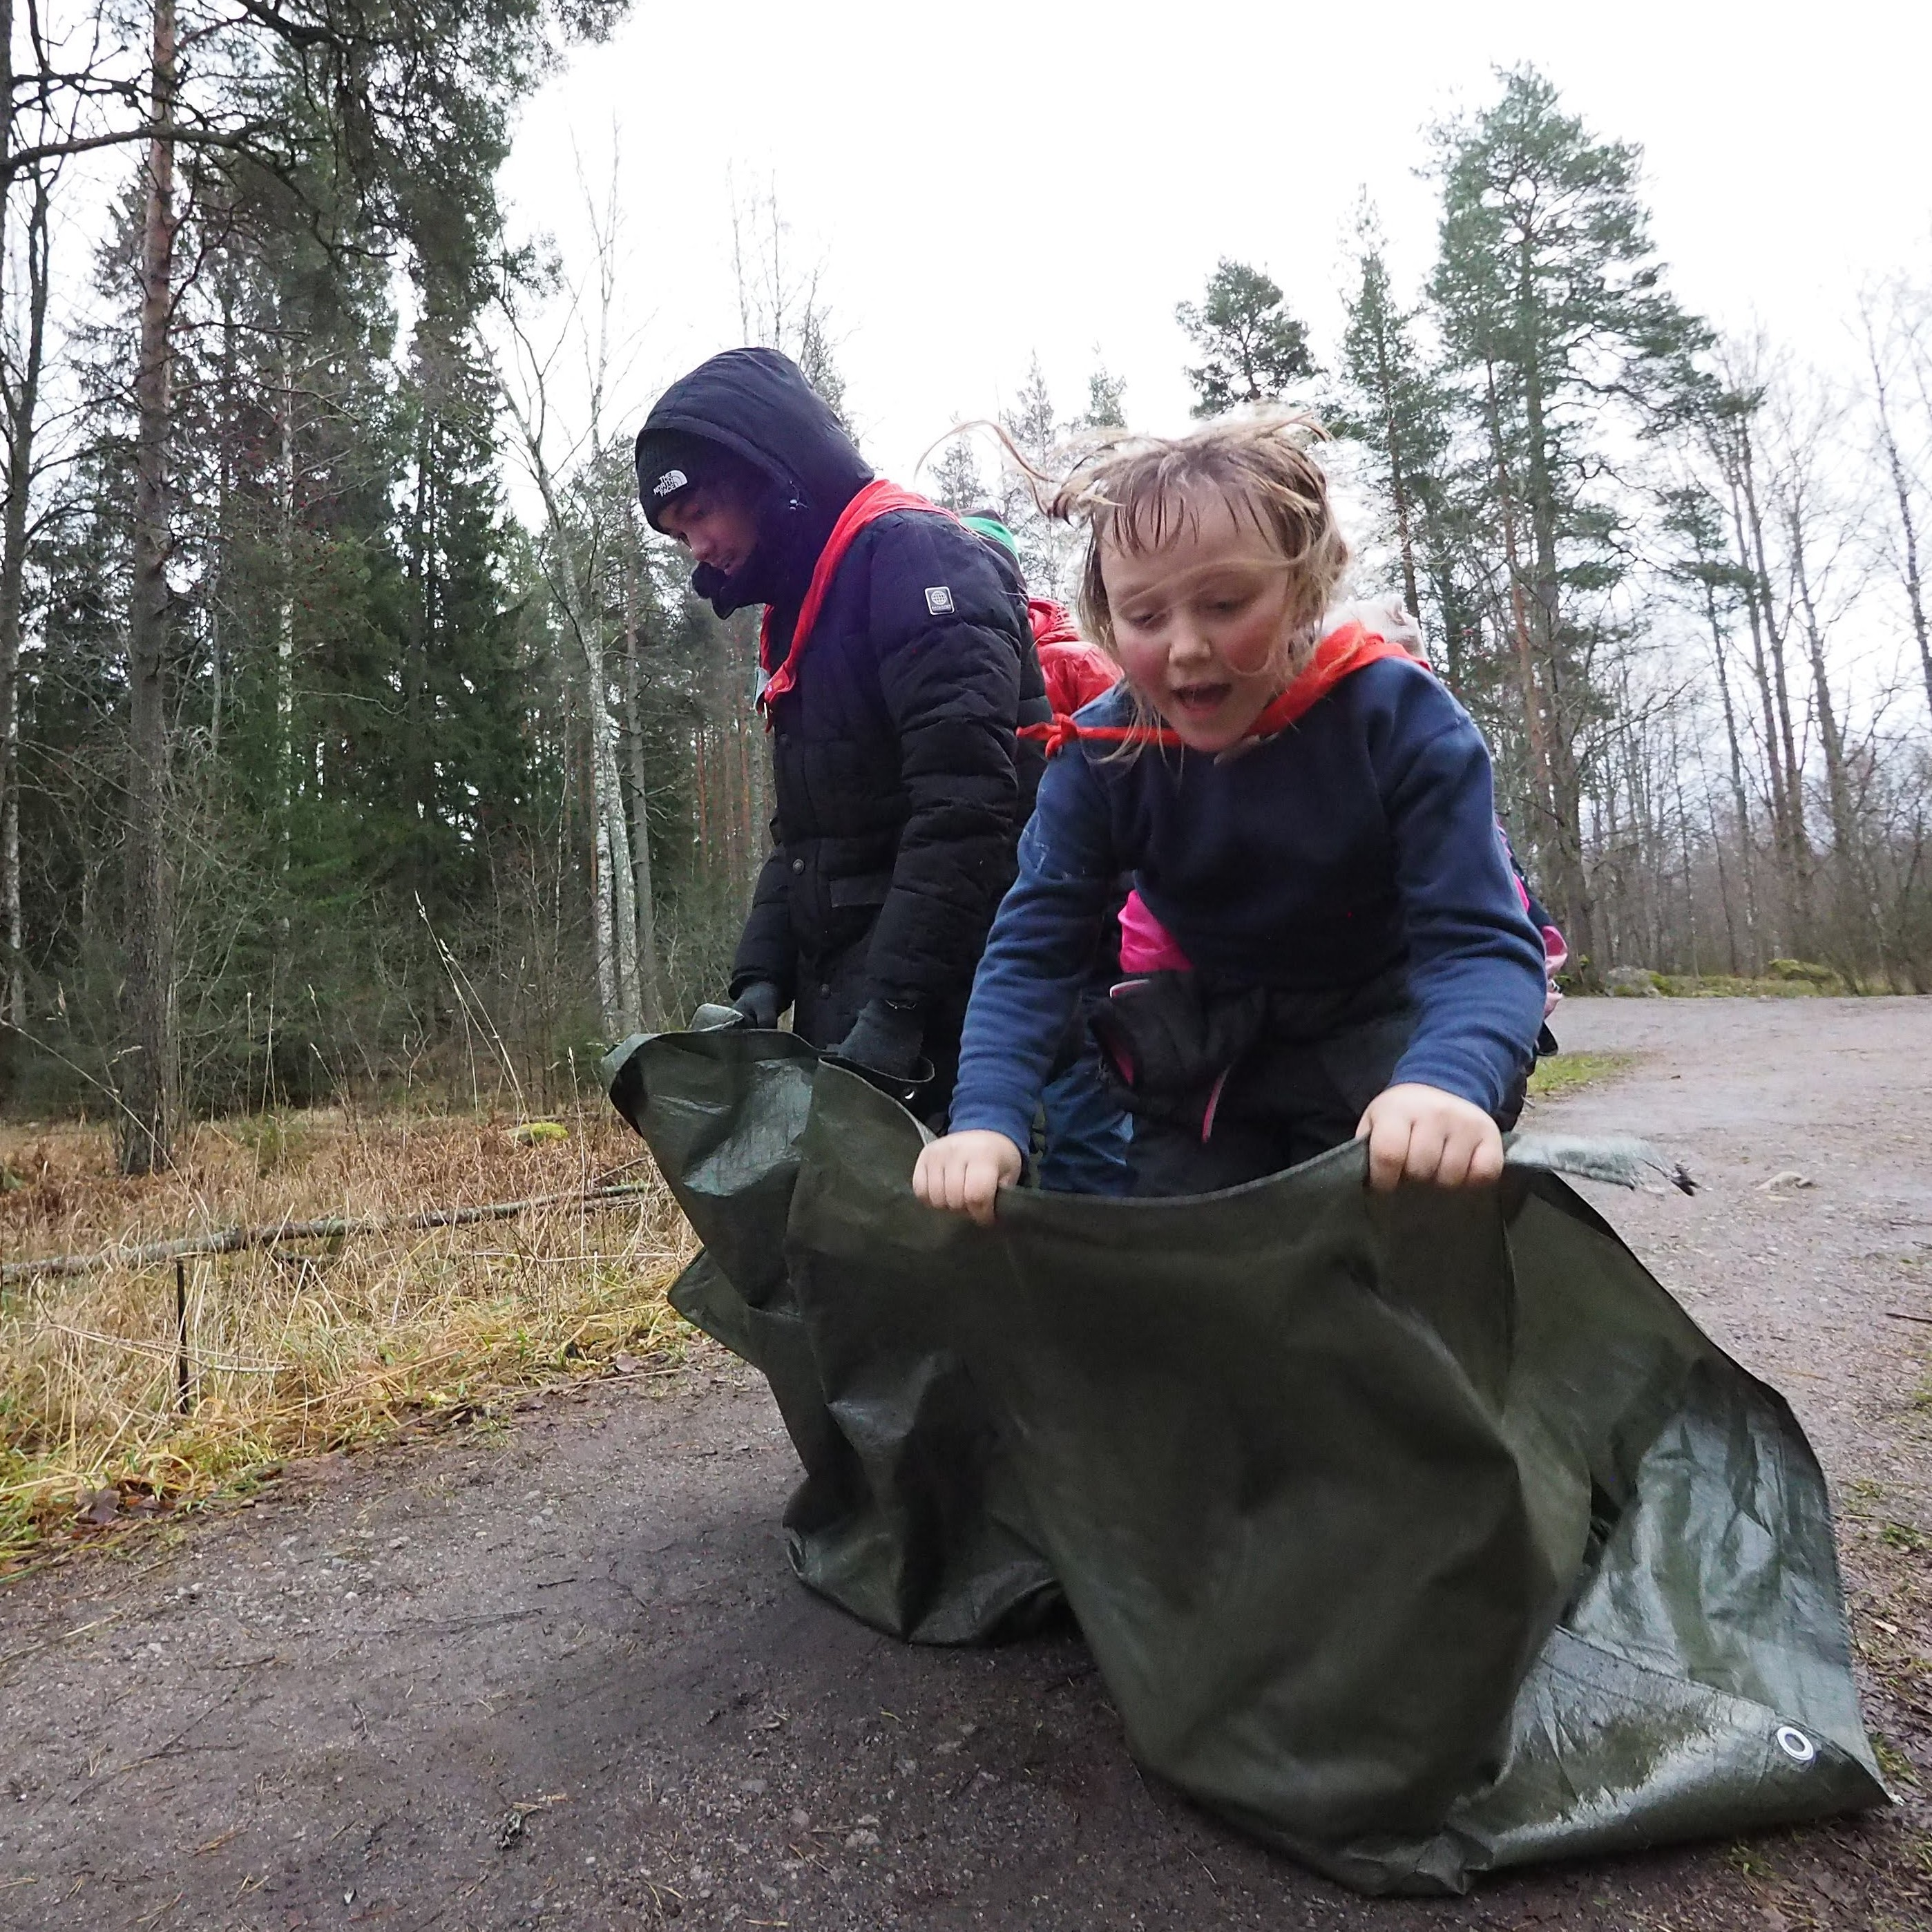
\includegraphics[width=.475\textwidth]{assets/meriharjuTaikamatto}\hfill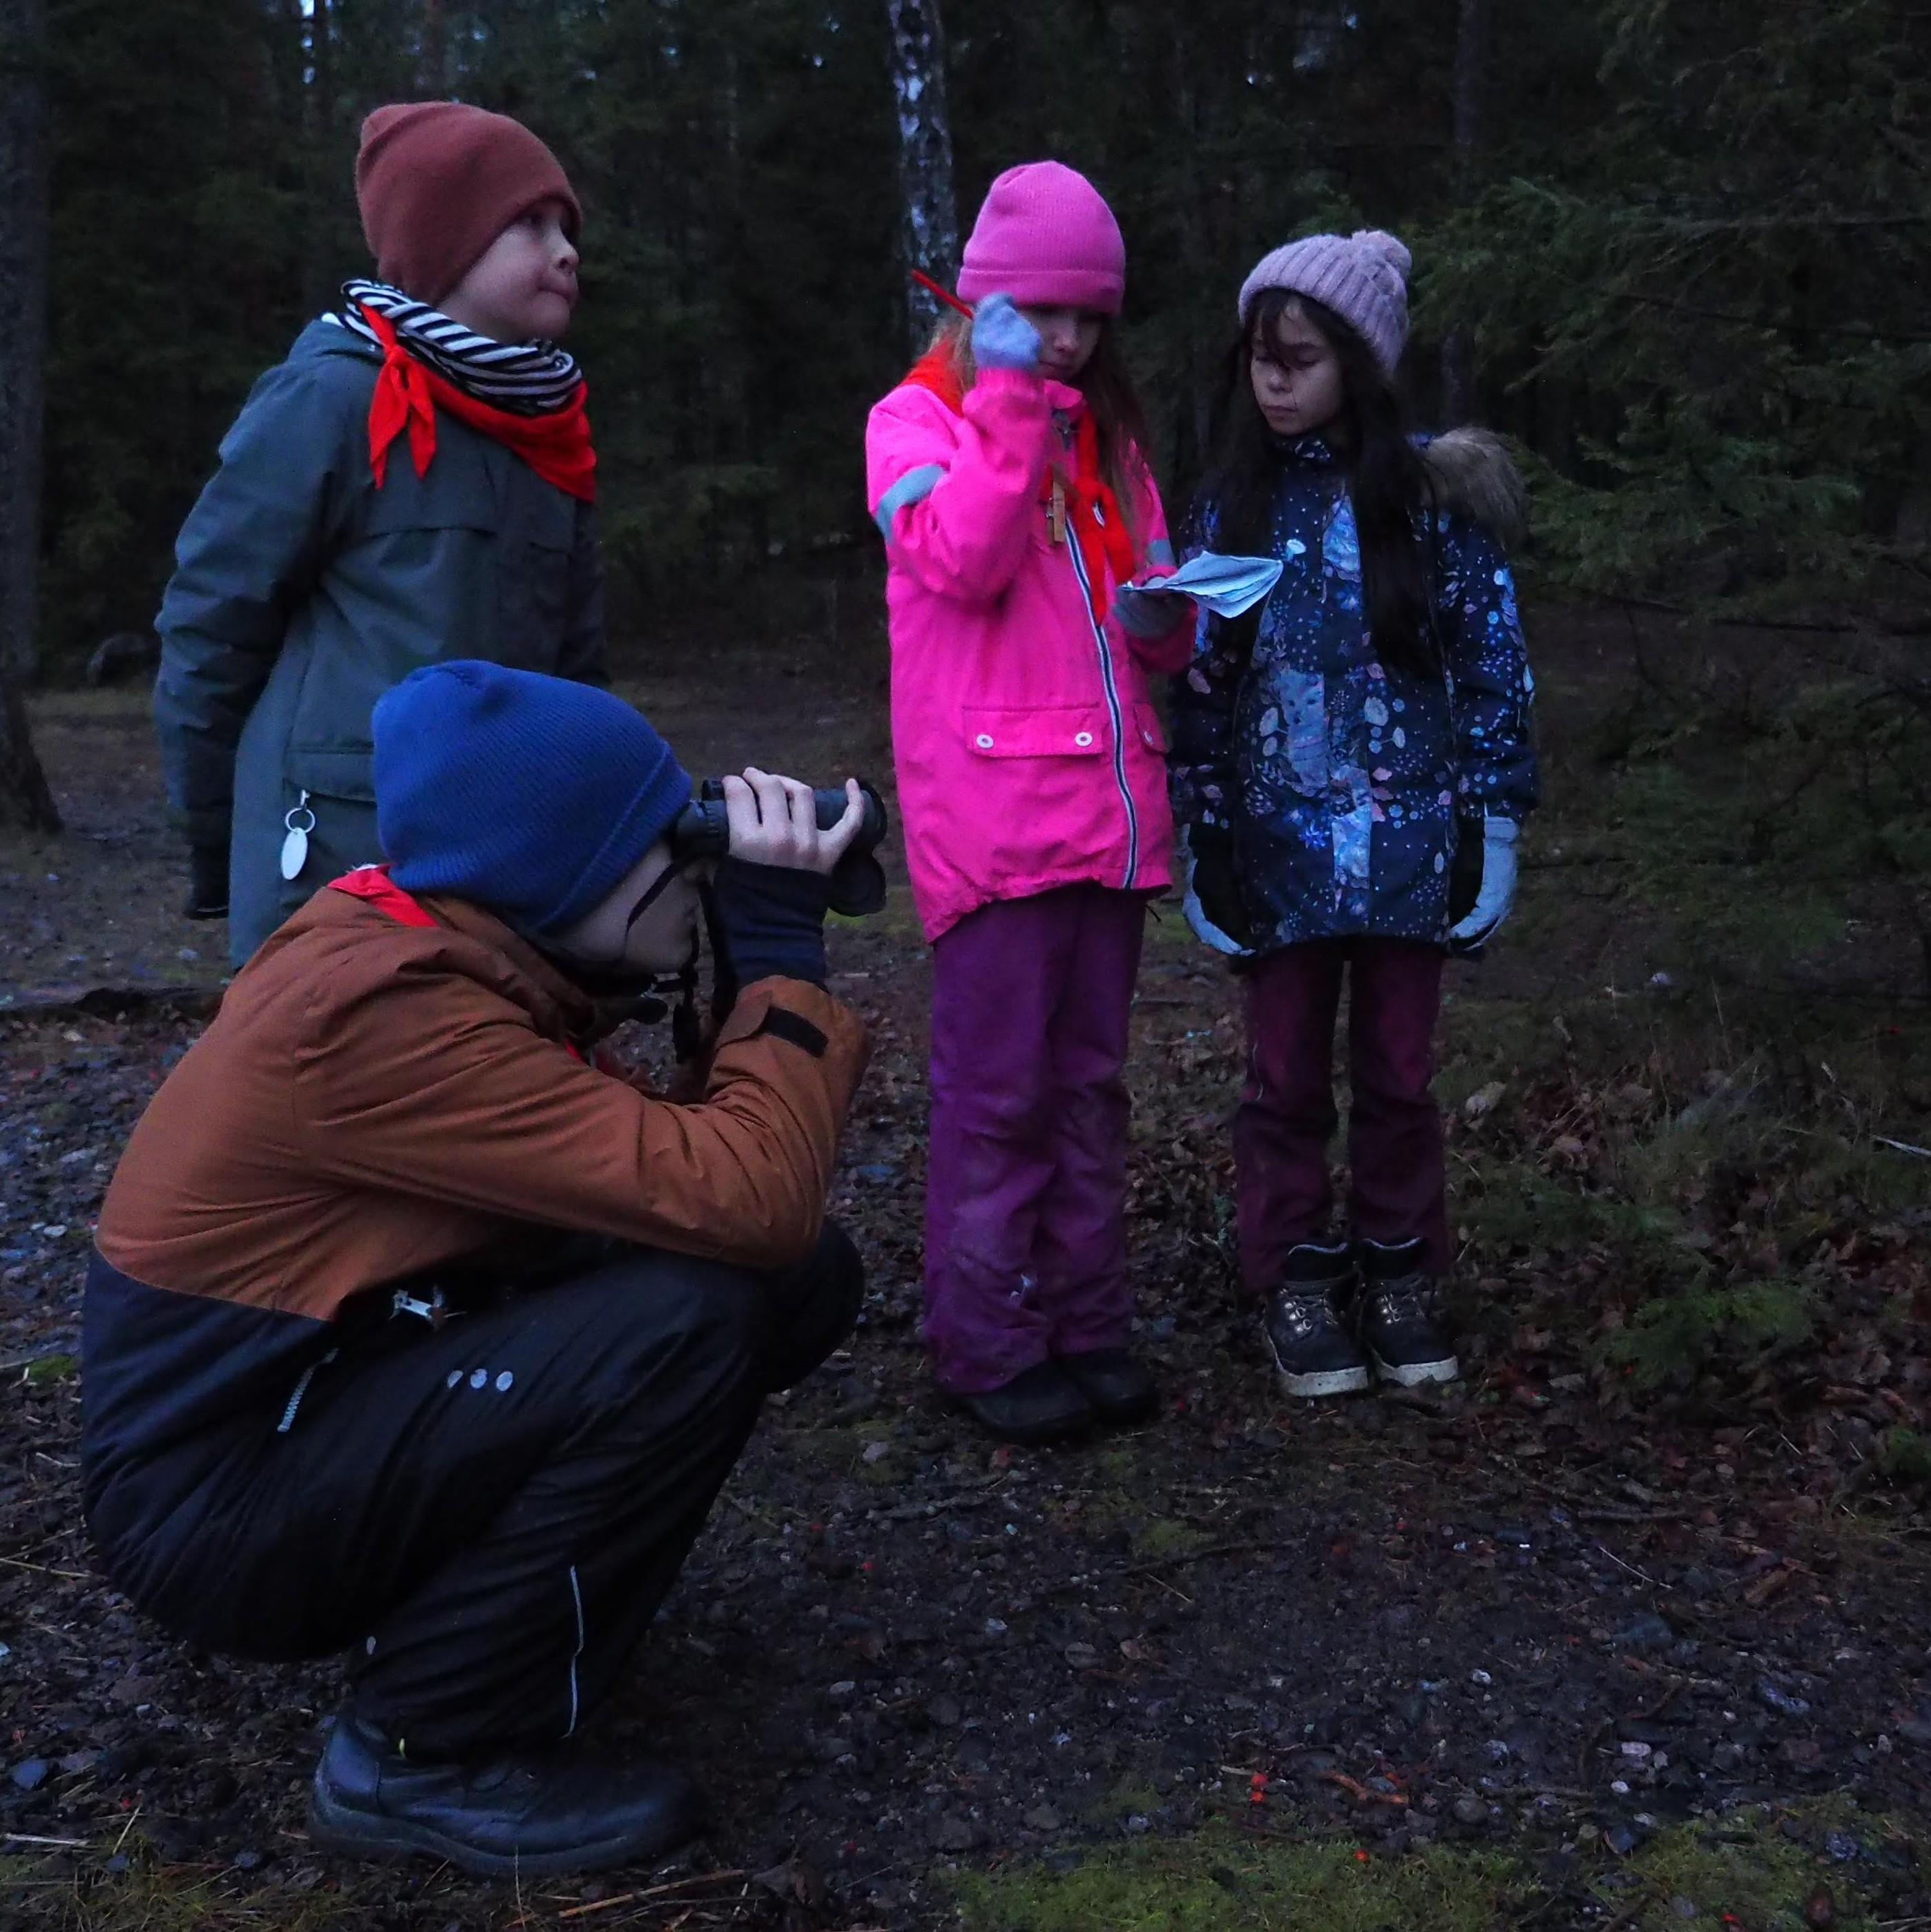
\includegraphics[width=.475\textwidth]{assets/meriharjuLinnut}
\caption{Neonvalo-vartio Kuusenalusmatto-rastilla ja Tyypit-vartio Poro, peura tai hirvi? -rastilla.}
\end{figure*}

Peräti 24 rusakkoa kokoontui jo tutuksi käyneellä bussilinja 560:n 
pysäkillä Kontulassa, josta matka jatkui kohti itää. Kävely Vuosaaren 
metroasemalta luontotalolle oli nuorempien retkeläisten mielestä 
jännittävä, kun viimeisellä kilometrillä ei ollutkaan enää 
katuvalaistusta. Tasku- ja otsalamput kaivettiinkin esiin hyvissä ajoin 
lyhyellä tauolla Sumujen sillalla. 

Kämpän pihalla vuorossa oli retkenjohtajan lyhyt ohjeistus ja Vene"-vartion 
leikkikimara ennen sisään siirtymistä ja majoittautumista: uniikki, 
sisäkissa"-ulkokissa ja lännen nopein. Kolkat yöpyisivät yhdessä 
huoneessa, seikkailijat ja tarpojat toisessa, samoajat ja Nonna kolmannessa ja 
muut johtajat neljännessä huoneessa. Retken kokonaisvahvuus oli 33 eli kaikki 
sänkypaikat paitsi yksi tulivat käytettyä.

Voileipäiltapalan jälkeen siirryttiinkin jo iltatoimille ja nukkumaan. Osa 
seikkailijoista ja tarpojista jäi vielä hetkeksi valvomaan takahuoneeseen ja 
osa johtajista kävi perjantaisaunassa.

Lauantaiaamu käynnistettiin kaurapuurolla ja pian oli aika suunnistukselle. 
Matkaan lähti viisi vartiota: Sudet, Neonvalo, Pupunkorvat, Tyypit ja 
S.U.P.E.R.G.A.L.A.K.T.I.S.E.T. F.E.M.I.N.I.S.T.I.M.A.R.S.U.T. (lyhyemmin 
S.G.F.M.). Rastikiertoon liittyi retken teemaan sopiva kehystarina, joka 
mukaili Marketta Pyysalon kertomusta \textit{Siili, jonka joulu herätti}. 

Suunistuksen ensimmäisellä rasteilla tunnistettiin eläinten lumijälkiä. 
Valitettavasti retkilauantaina ei vielä lunta maassa ollut, minkä vuoksi 
jälkien tunnistus tapahtui puhelimen näytöltä. Toisella rastilla vartion 
tehtävänä oli edetä pressun päällä rastihenkilön määräämä matka ja 
kolmannella laulaa joululauluja, joissa esiintyi tiettyjä sanoja. Neljäs 
rasti sijaitsi Niemenapajalla, jossa vartio etsi kertakäyttölusikoita 
maastosta.

\begin{figure*}[!t]
\centering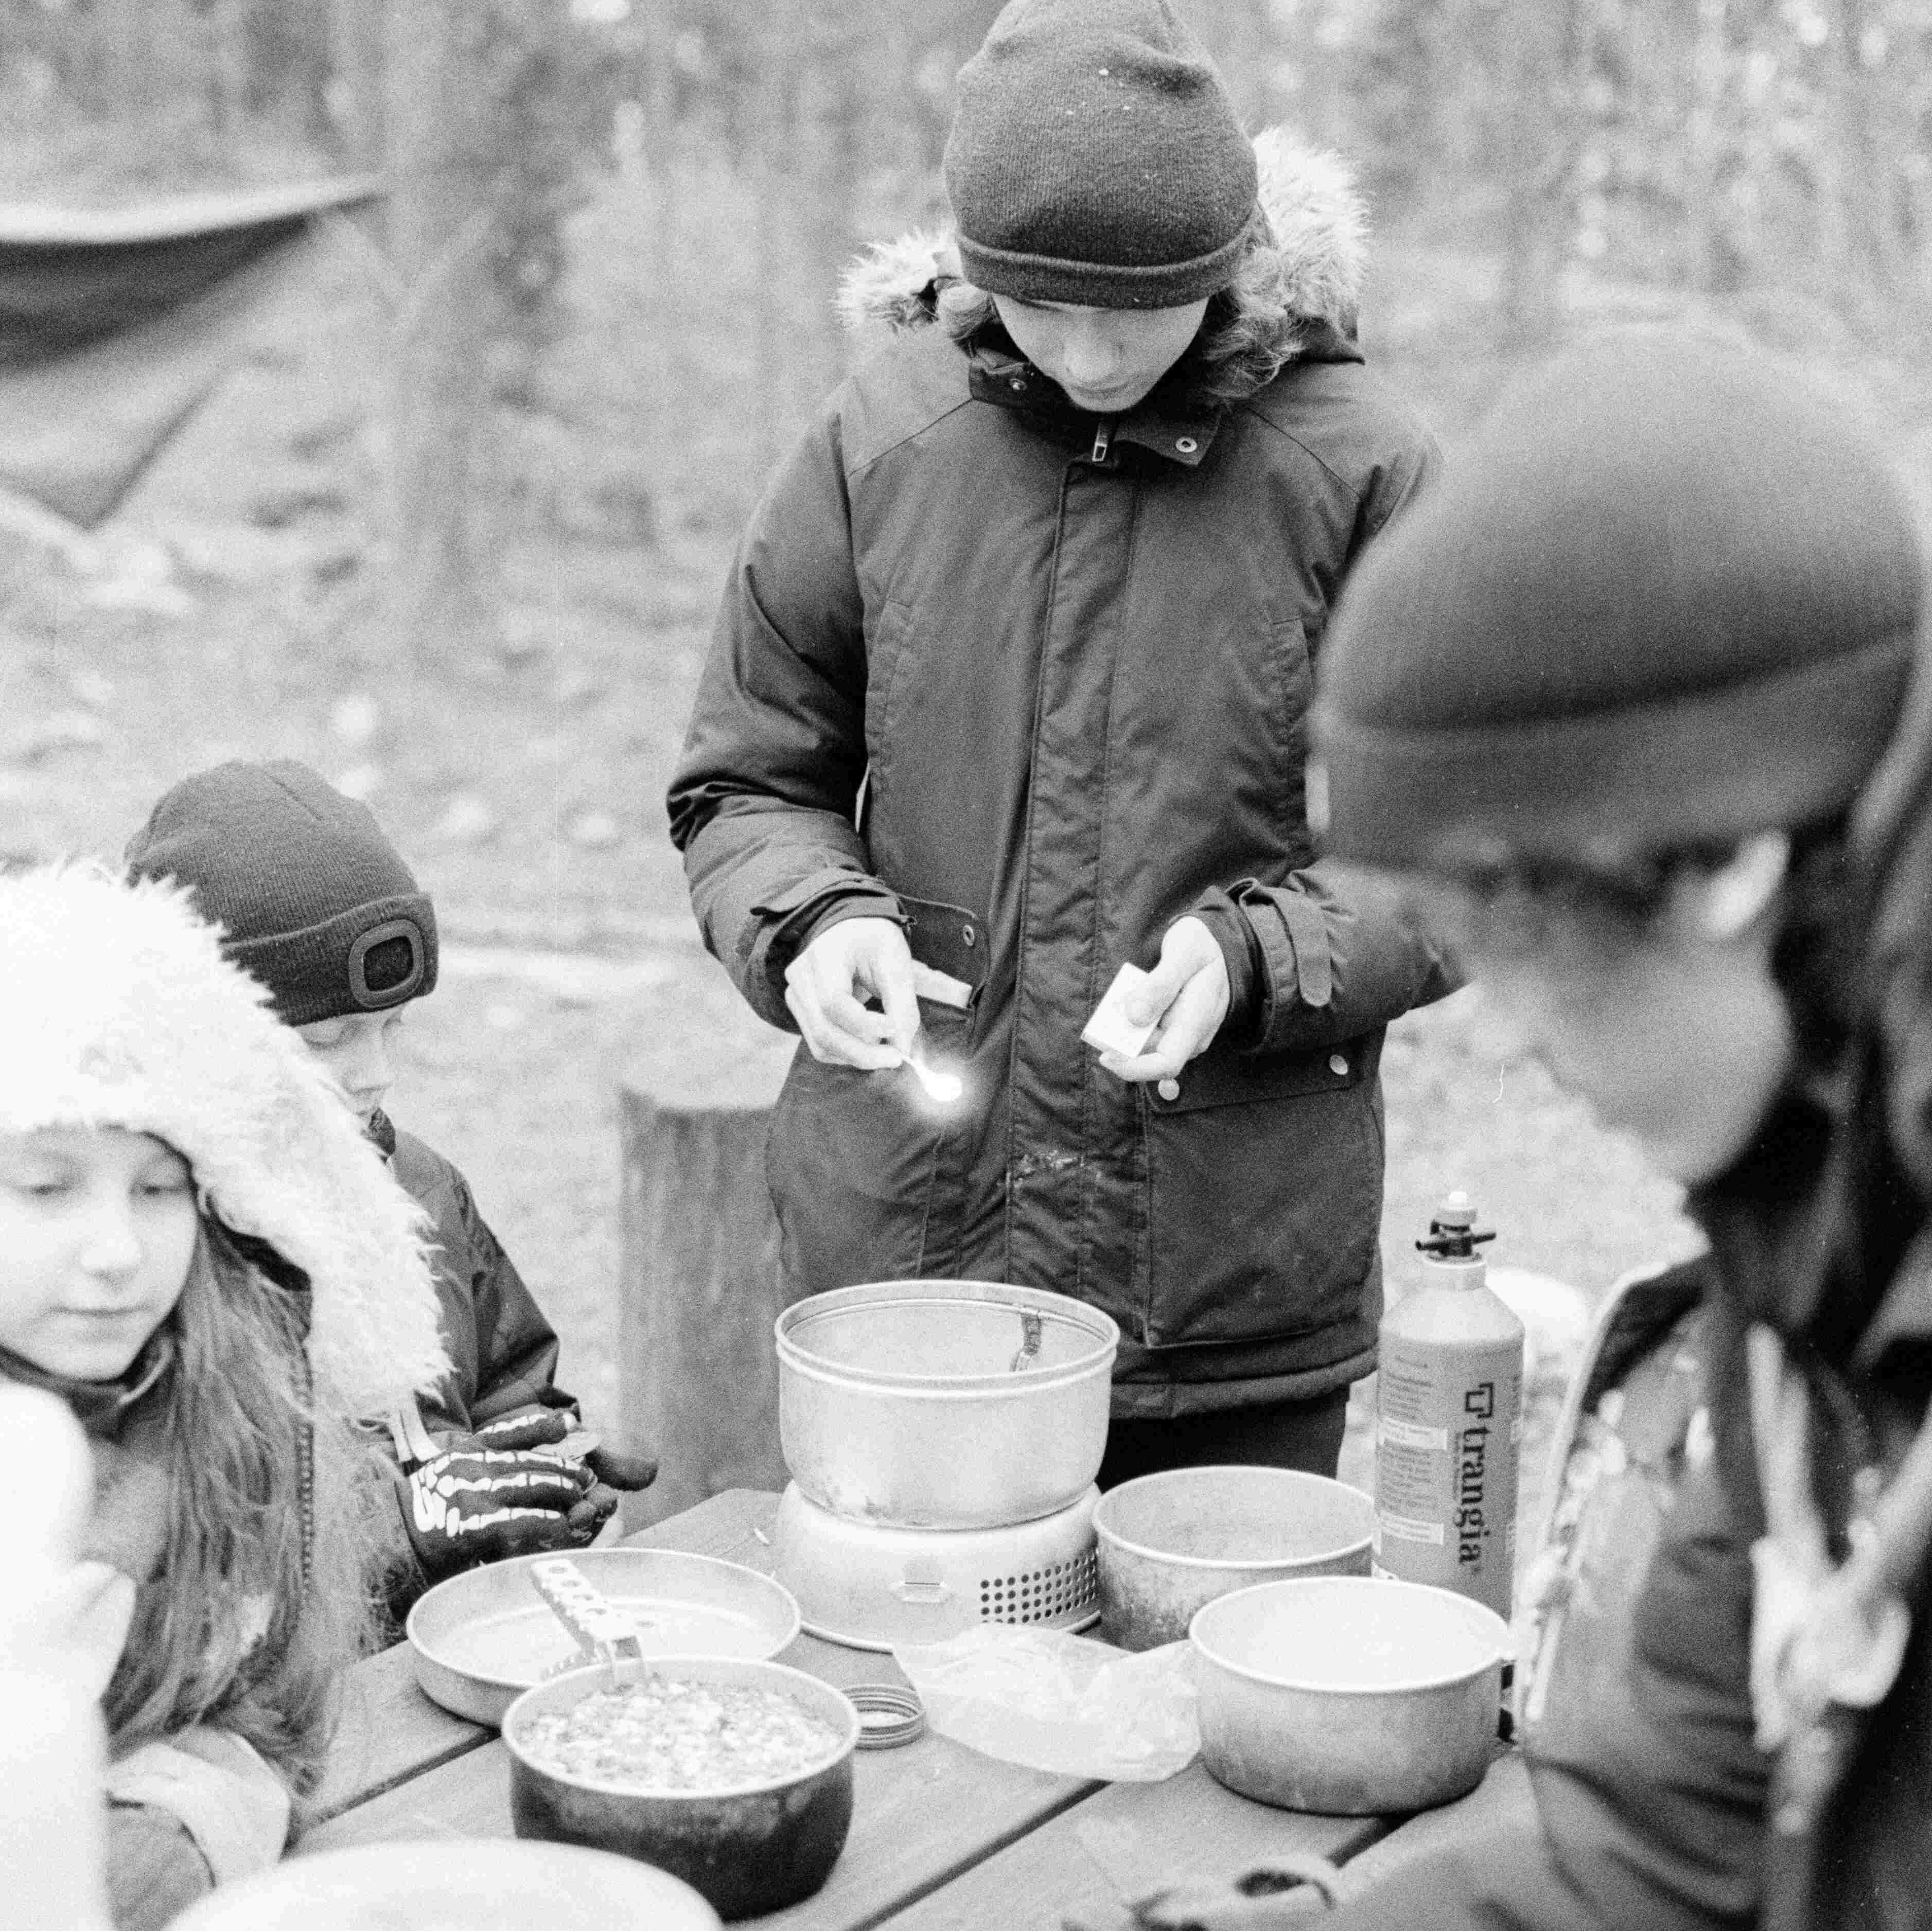
\includegraphics[width=.475\textwidth]{assets/meriharjuRuoka1}\hfill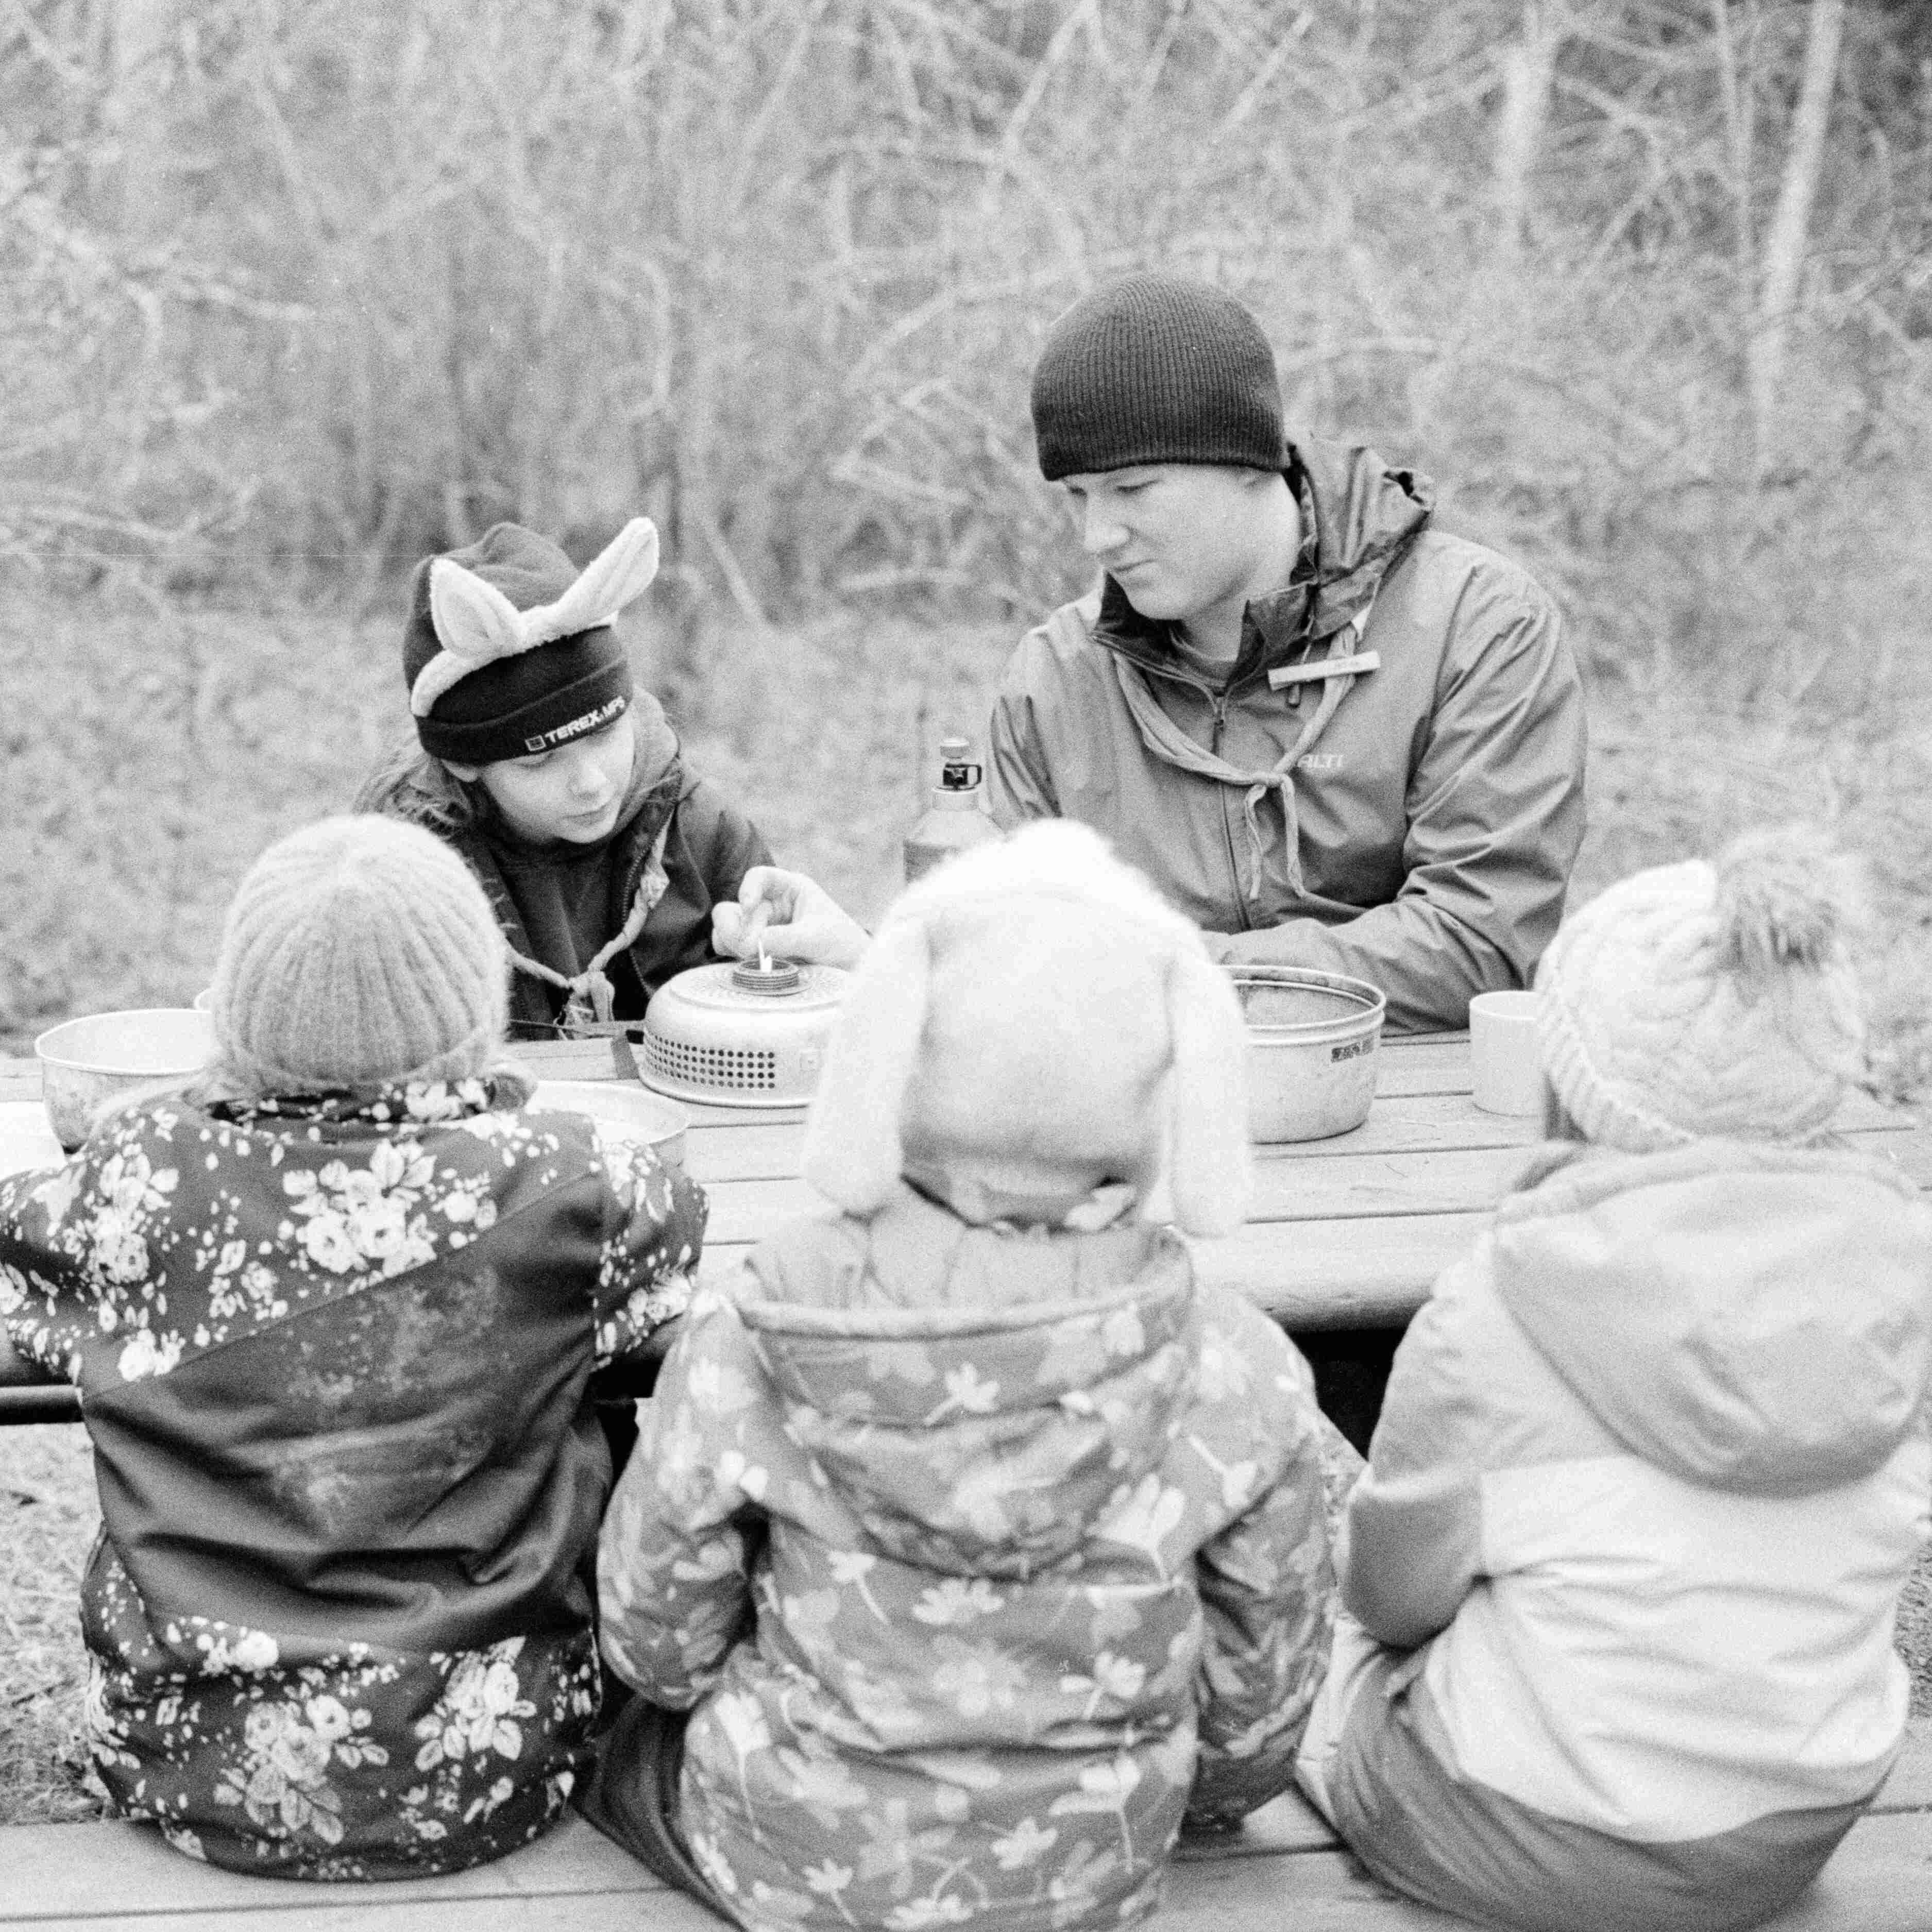
\includegraphics[width=.475\textwidth]{assets/meriharjuRuoka2}
\caption{Sudet- ja Pupunkorvat -vartiot ruokarastilla.}
\end{figure*}

Vielä oli kaksi rastia jäljellä, mutta ennen niitä vartiot valmistivat 
itselleen maittavan trangialounaan: tonnikalanuudeleita, nams! Tässä 
vaiheessa alkoi sataa vähän räntää, mutta se ei vartoiden menoa haitannut. 
Kuudennella rastilla tehtiin iso merimiessolmu ja seitsemännellä rastilla 
tunnistettiin eläimiä. Maalitehtävä oli muita rastitehtäviä huomattavasti 
haastavampi, kun vartioiden piti yhdistää maakunnan vaakuna sitä vastaavaan 
maakuntamaaeläimeen, "=lintuun tai "=kalaan. 

Vaikka varsinaisia suunnistuksia ei viime lippukuntaretkillä ole ollutkaan 
ohjelmassa, kaikki vartiot löysivät hienosti kaikille rasteille. Seitsemän 
rastin, vajaan kahdeksan kilometrin suunnistukseen meni nopeimmalta vartiolta 
noin viisi tuntia ja hitaimmalta kuusi tuntia. Nopeudesta ei saanut pisteitä, 
mutta rastitehtävät pisteytettiin -- löydät vartoiden pisteytykset 
jutun lopun taulukosta. Onneksi olkoon, Tyypit!

Samaa vauhtia kuin vartiot saapuivat suunnistuksen maaliin vartiot alkoivat 
suunnitella omia piparkakkutalojaan. Kukin vartio sai käyttöönsä kokonaisen 
kilon piparkakkutaikinaa, josta tarkoituksena oli rakentaan kullekin vartiolle 
mieluisa teos. Varsin moni vartio rakensi perinteikästä piparkakkutaloa 
mukailevan rakennelman, mutta myös jännittävämpiä ratkaisuja kuten 
piparkakkunelitahokas ja piparkakkupelikortit nähtiin. Myös teokset 
pisteytettiin.

\begin{figure*}[!t]
\centering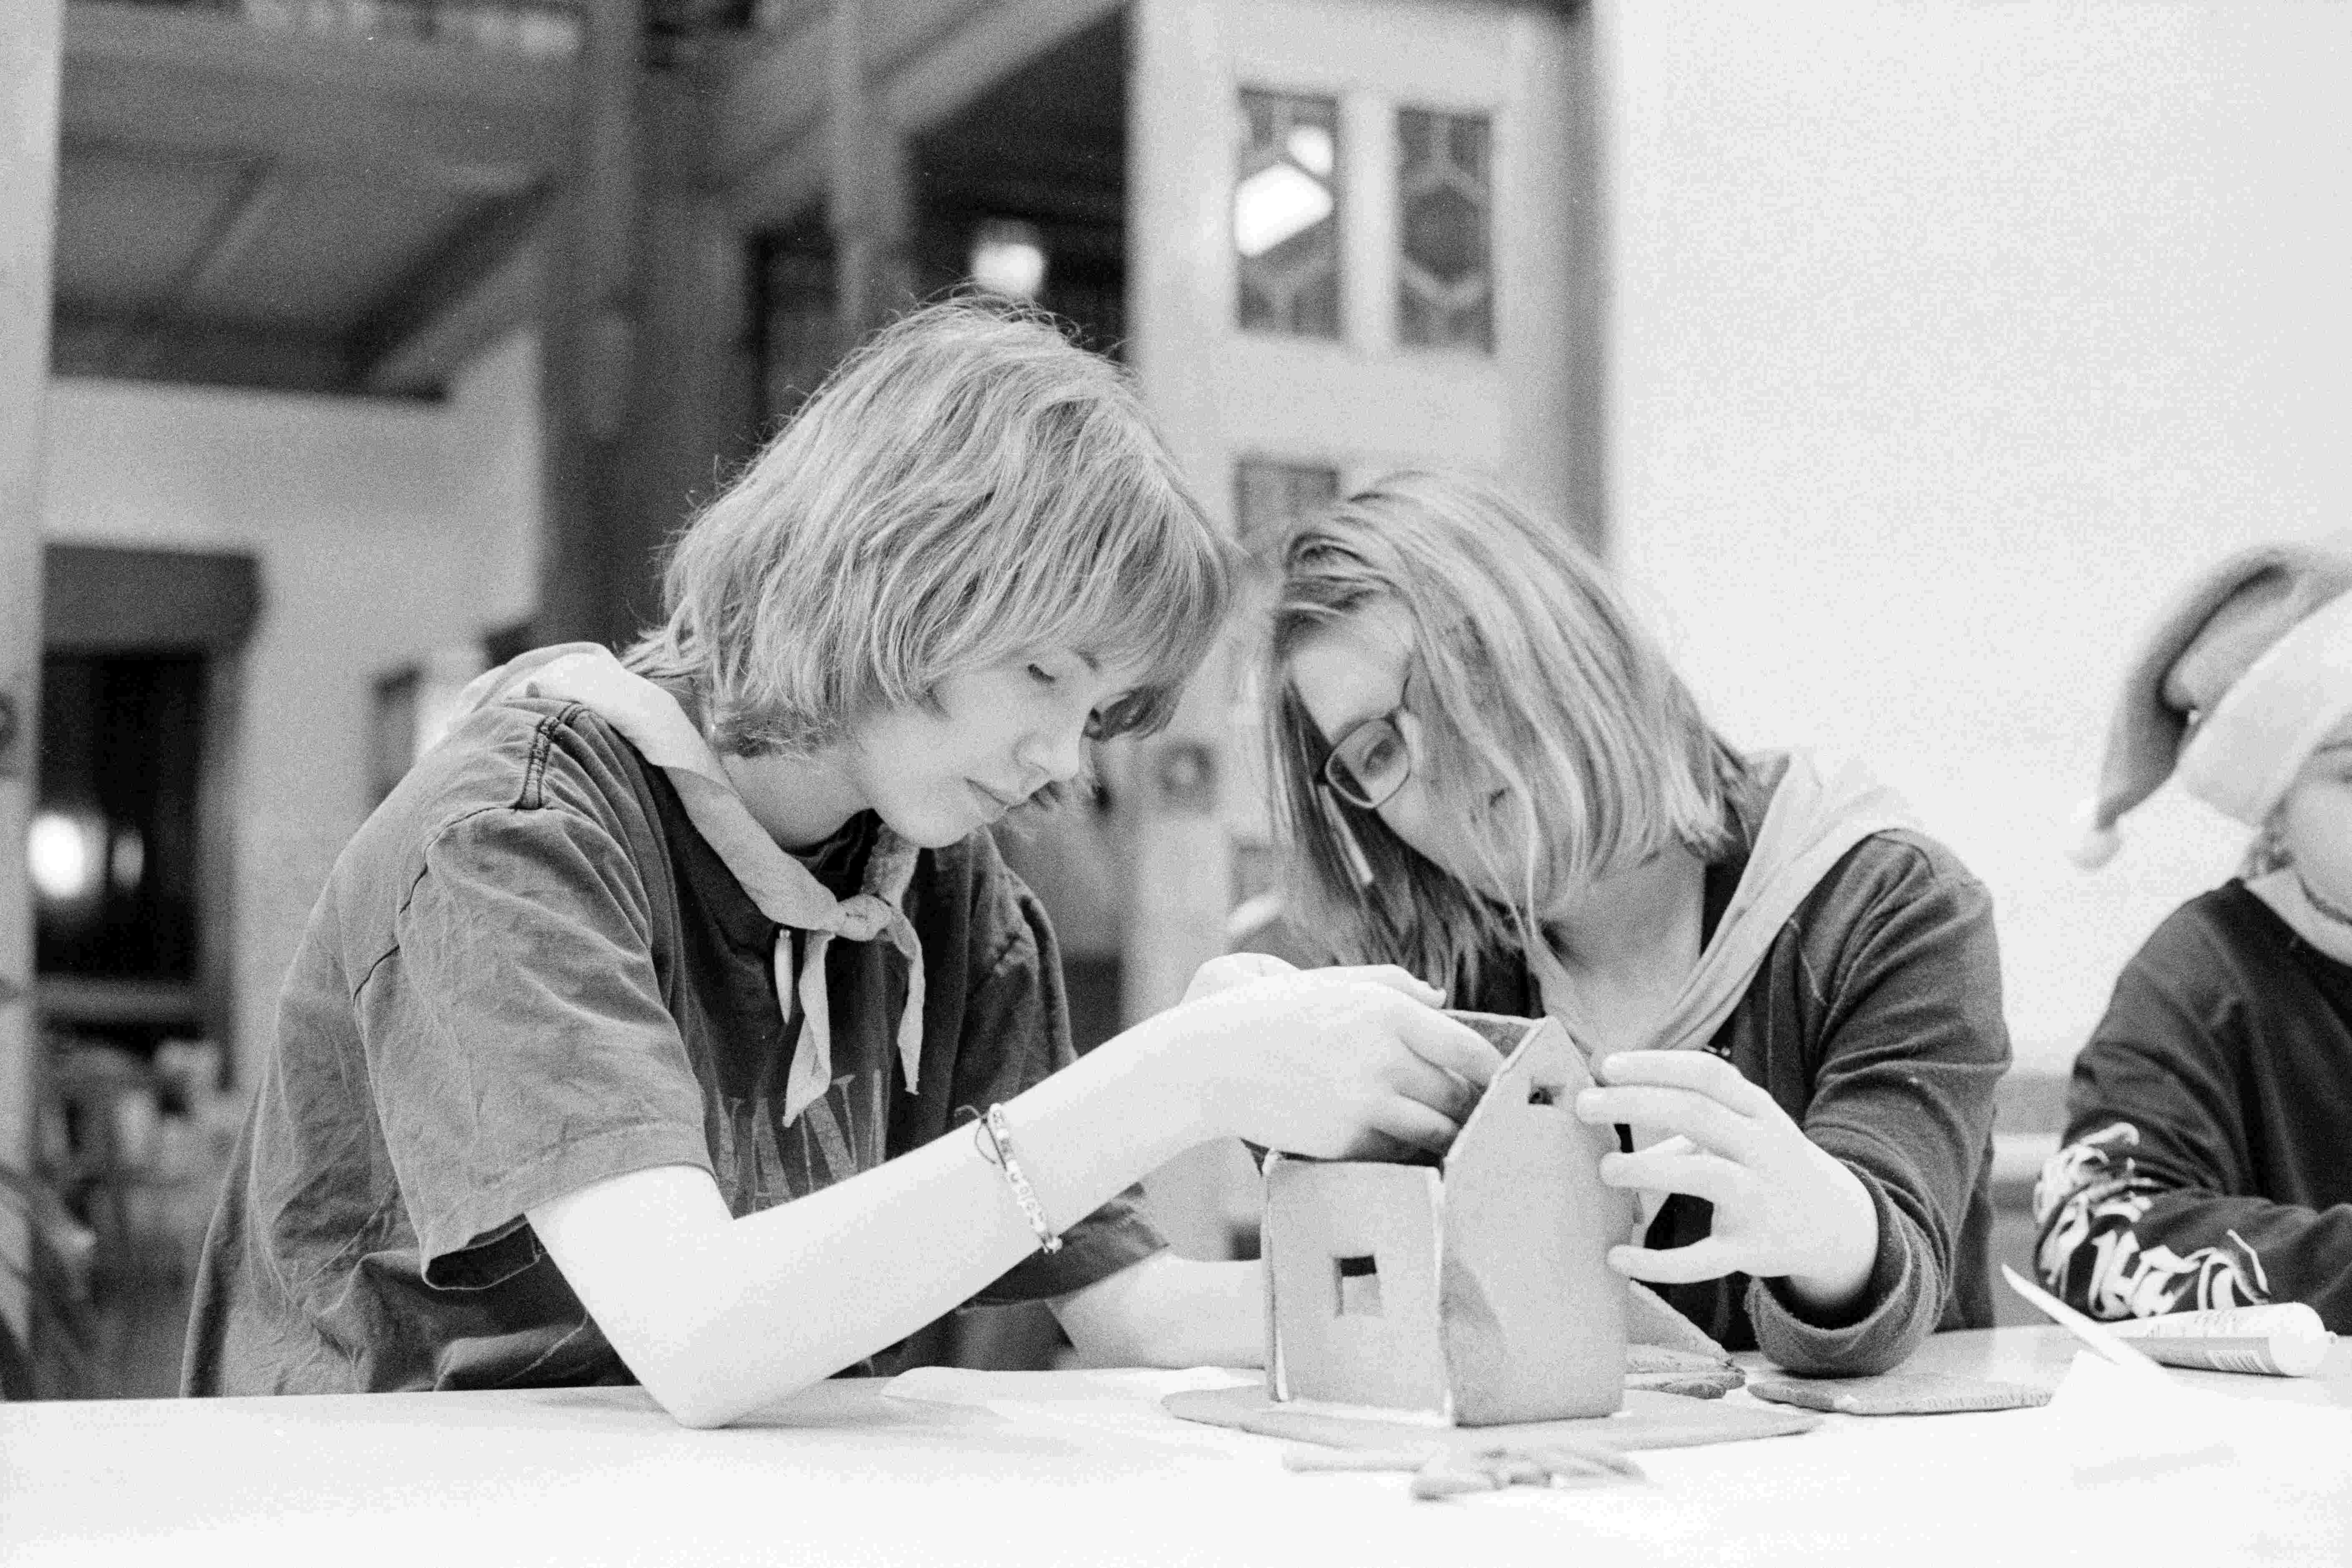
\includegraphics[width=\textwidth,trim={0 0 0 5cm},clip]{assets/meriharjuPipari}
\caption{S.U.P.E.R.G.A.L.A.K.T.I.S.E.T. F.E.M.I.N.I.S.T.I.M.A.R.S.U.T. -vartio rakentamassa piparkakkutaloa.}
\end{figure*}

\begin{table*}[b]\centering\small
\begin{tabular}{|l|c|c|c|c|c|}
\hline
 & \textbf{Tyypit} & 
\begin{tabular}[x]{@{}c@{}}\textbf{Pupun-}\\\textbf{korvat}\end{tabular} & 
\begin{tabular}[x]{@{}c@{}}\textbf{Neon-}\\\textbf{valo}\end{tabular} & 
\textbf{Sudet} & \textbf{S.G.F.M.} \\ \hline
\textbf{Lumijälkiä} & 3,00 & 3,00 & 1,00 & 3,00 & 5,00 \\ \hline
\textbf{Kuusenalusmatto} & 13,12 & 12,14 & 11,82 & 11,46 & 0,00 \\ \hline
\textbf{Kauneimmat joululaulut} & 10,00 & 8,00 & 7,00 & 2,00 & 6,00 \\ \hline
\begin{tabular}[x]{@{}c@{}}\textbf{Pata-himmeli 
ja}\\\textbf{ruutu-kranssi}\end{tabular} & 3,00 & 5,00 & 3,00 & 4,00 & 5,00 \\ 
\hline
\textbf{Joulurusetti} & 5,00 & 5,00 & 4,00 & 4,00 & 5,00 \\ \hline
\textbf{Poro, peura tai hirvi?} & 4,00 & 6,00 & 3,00 & 5,50 & 3,00 \\ \hline
\textbf{Joulun taikaa} & 25,00 & 12,50 & 25,00 & 12,50 & 12,50 \\ \hline
\textbf{Piparkakkutalot} & 30,00 & 35,00 & 24,00 & 35,00 & 37,00 \\ \hline \hline
 & 93,12 & 86,64 & 78,82 & 77,46 & 73,50 \\ \hline
\end{tabular}
\end{table*}

Piparkakkuteosten osien paistuessa syötiin herkullista kanapataa. 
Päivällisen jälkeen halukkaat kävivät saunomassa muiden laulaessa 
joululauluja ja koristellessa teoksiaan. Iltapalaksi oli jotain hieman 
erikoisempaa: nyhtöleipää, keksejä ja paukkumaissia!

Sunnuntaiaamu käytettiin pakkaamiseen ja siivoamiseen. Uusille kolkille 
järjestettiin kolkkakoe, jonka kaikki kolme kokelasta läpäisivät. Lounaaksi 
juuri ennen joulujuhlaa syötiin riisipuuroa. 

\begin{figure*}[p]
\centering
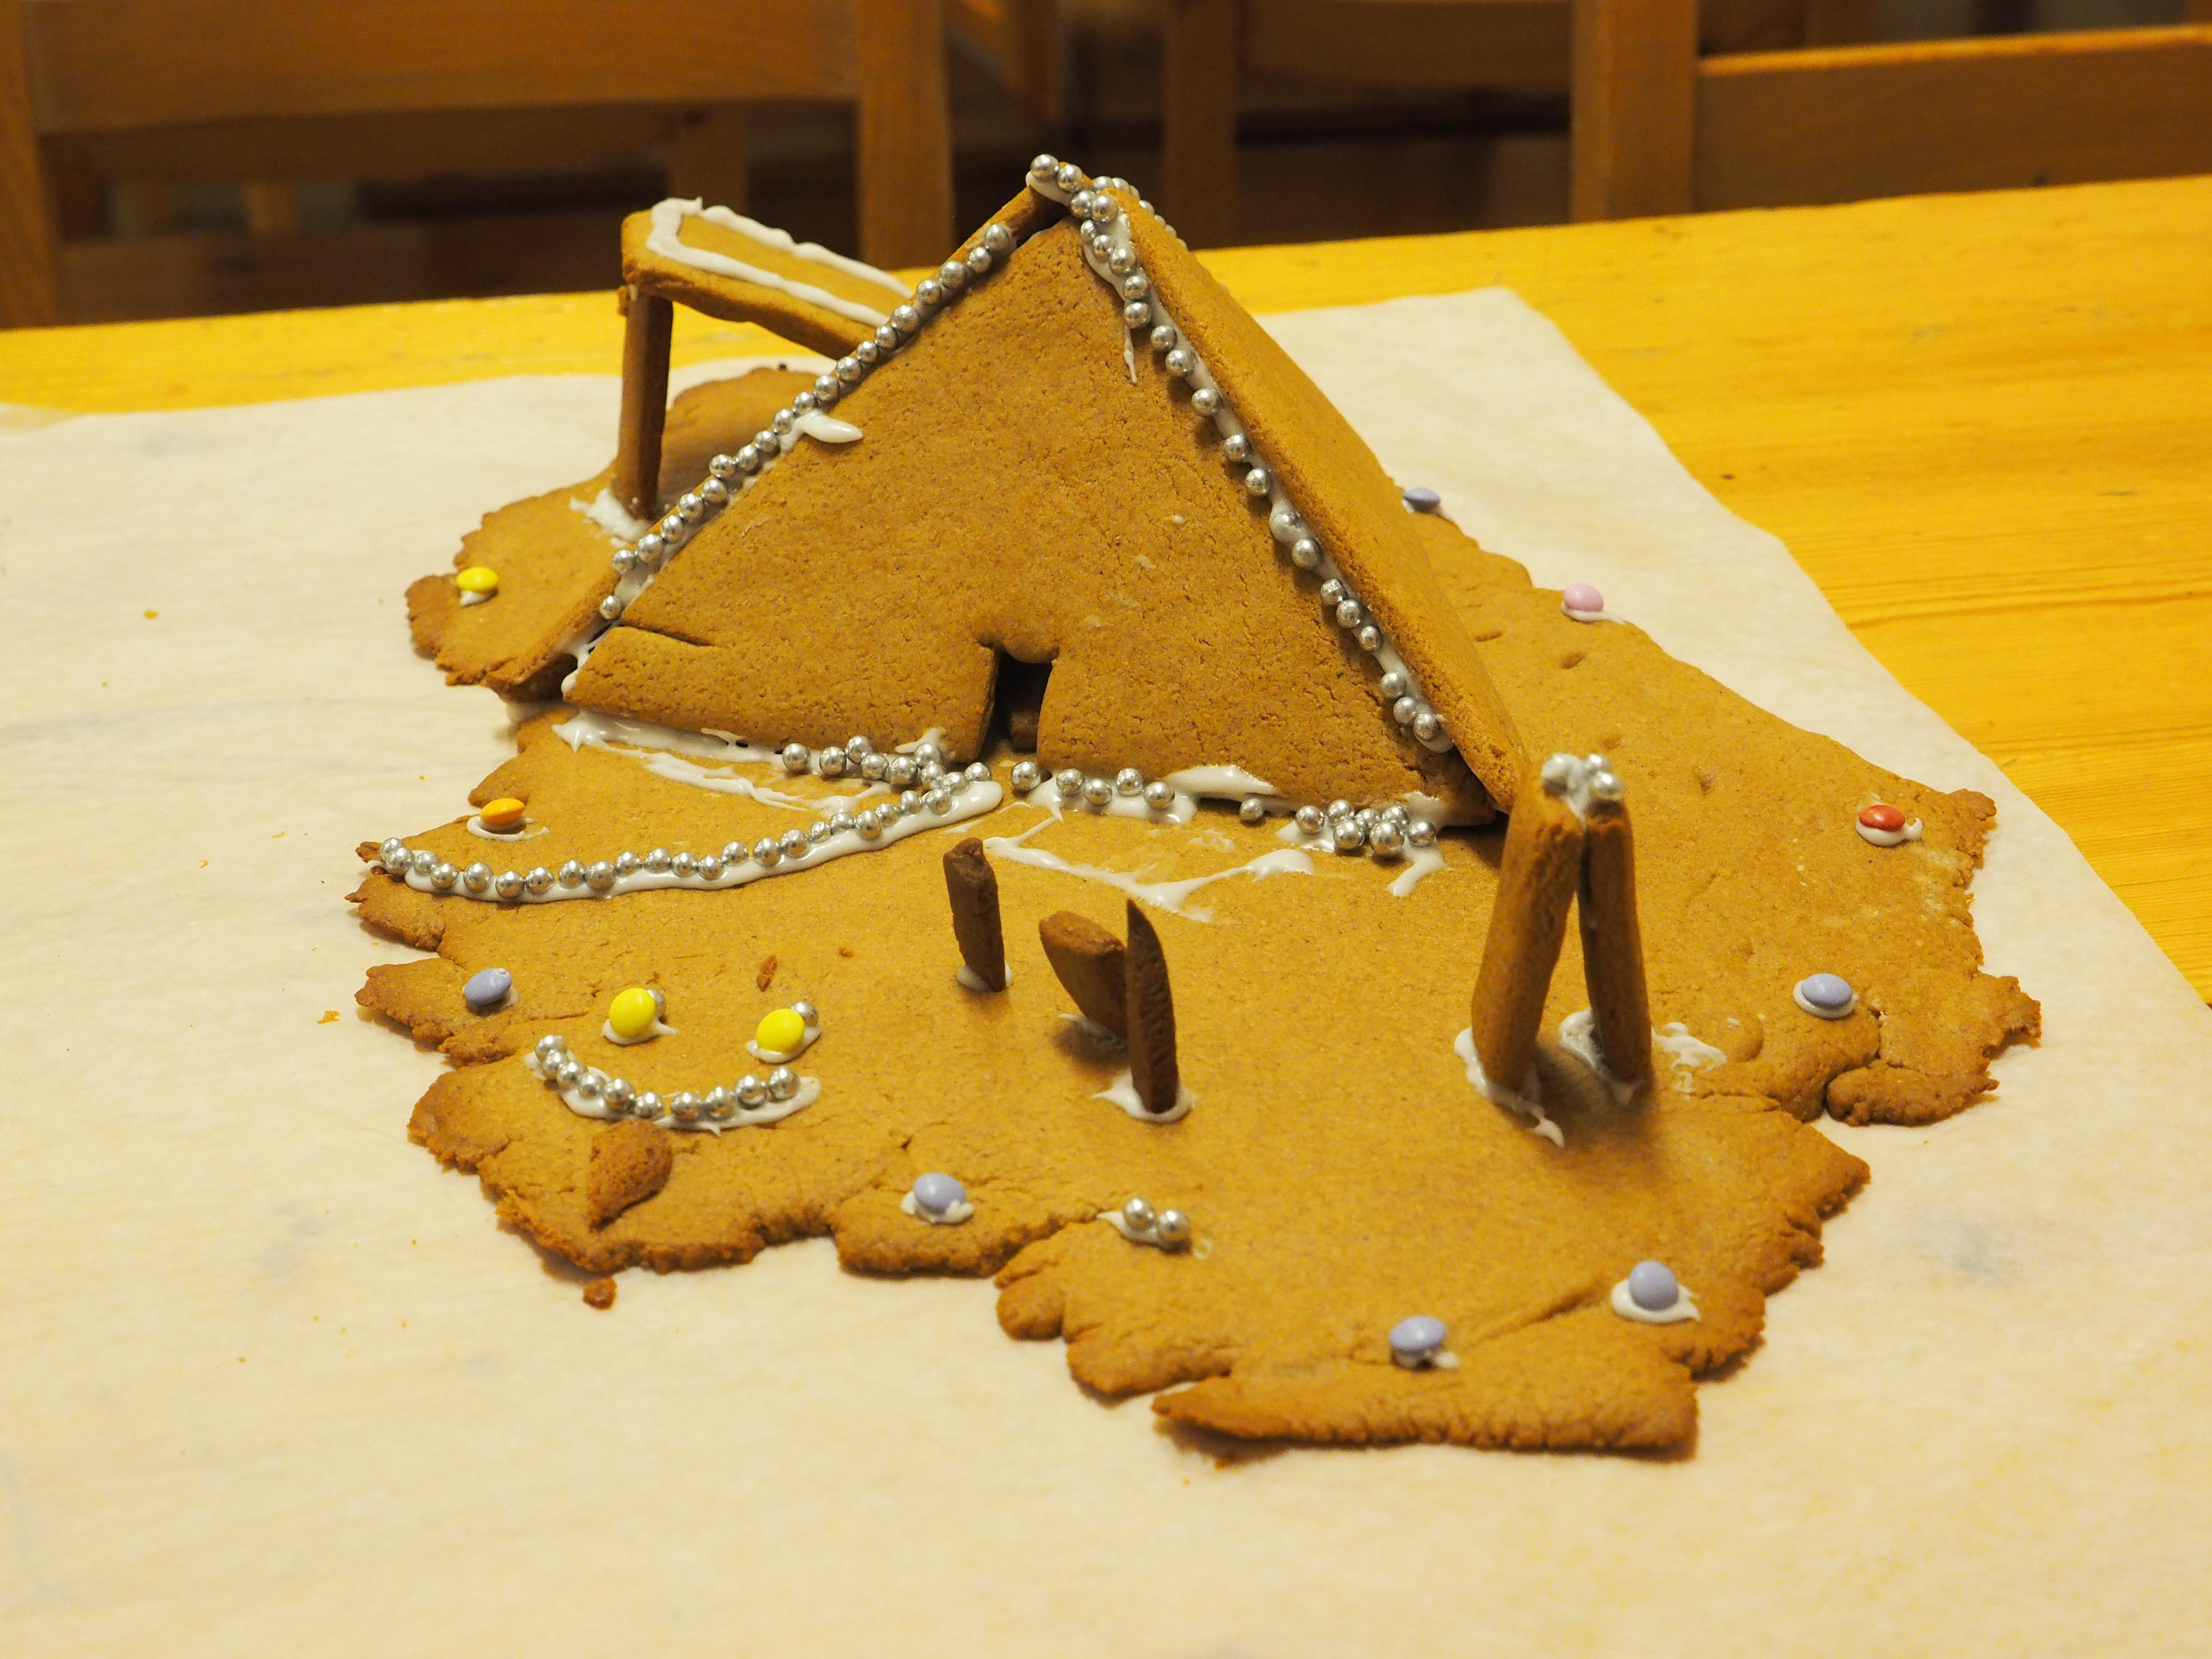
\includegraphics[width=.475\textwidth,height=.475\textwidth,keepaspectratio]{assets/pipari1}\hfill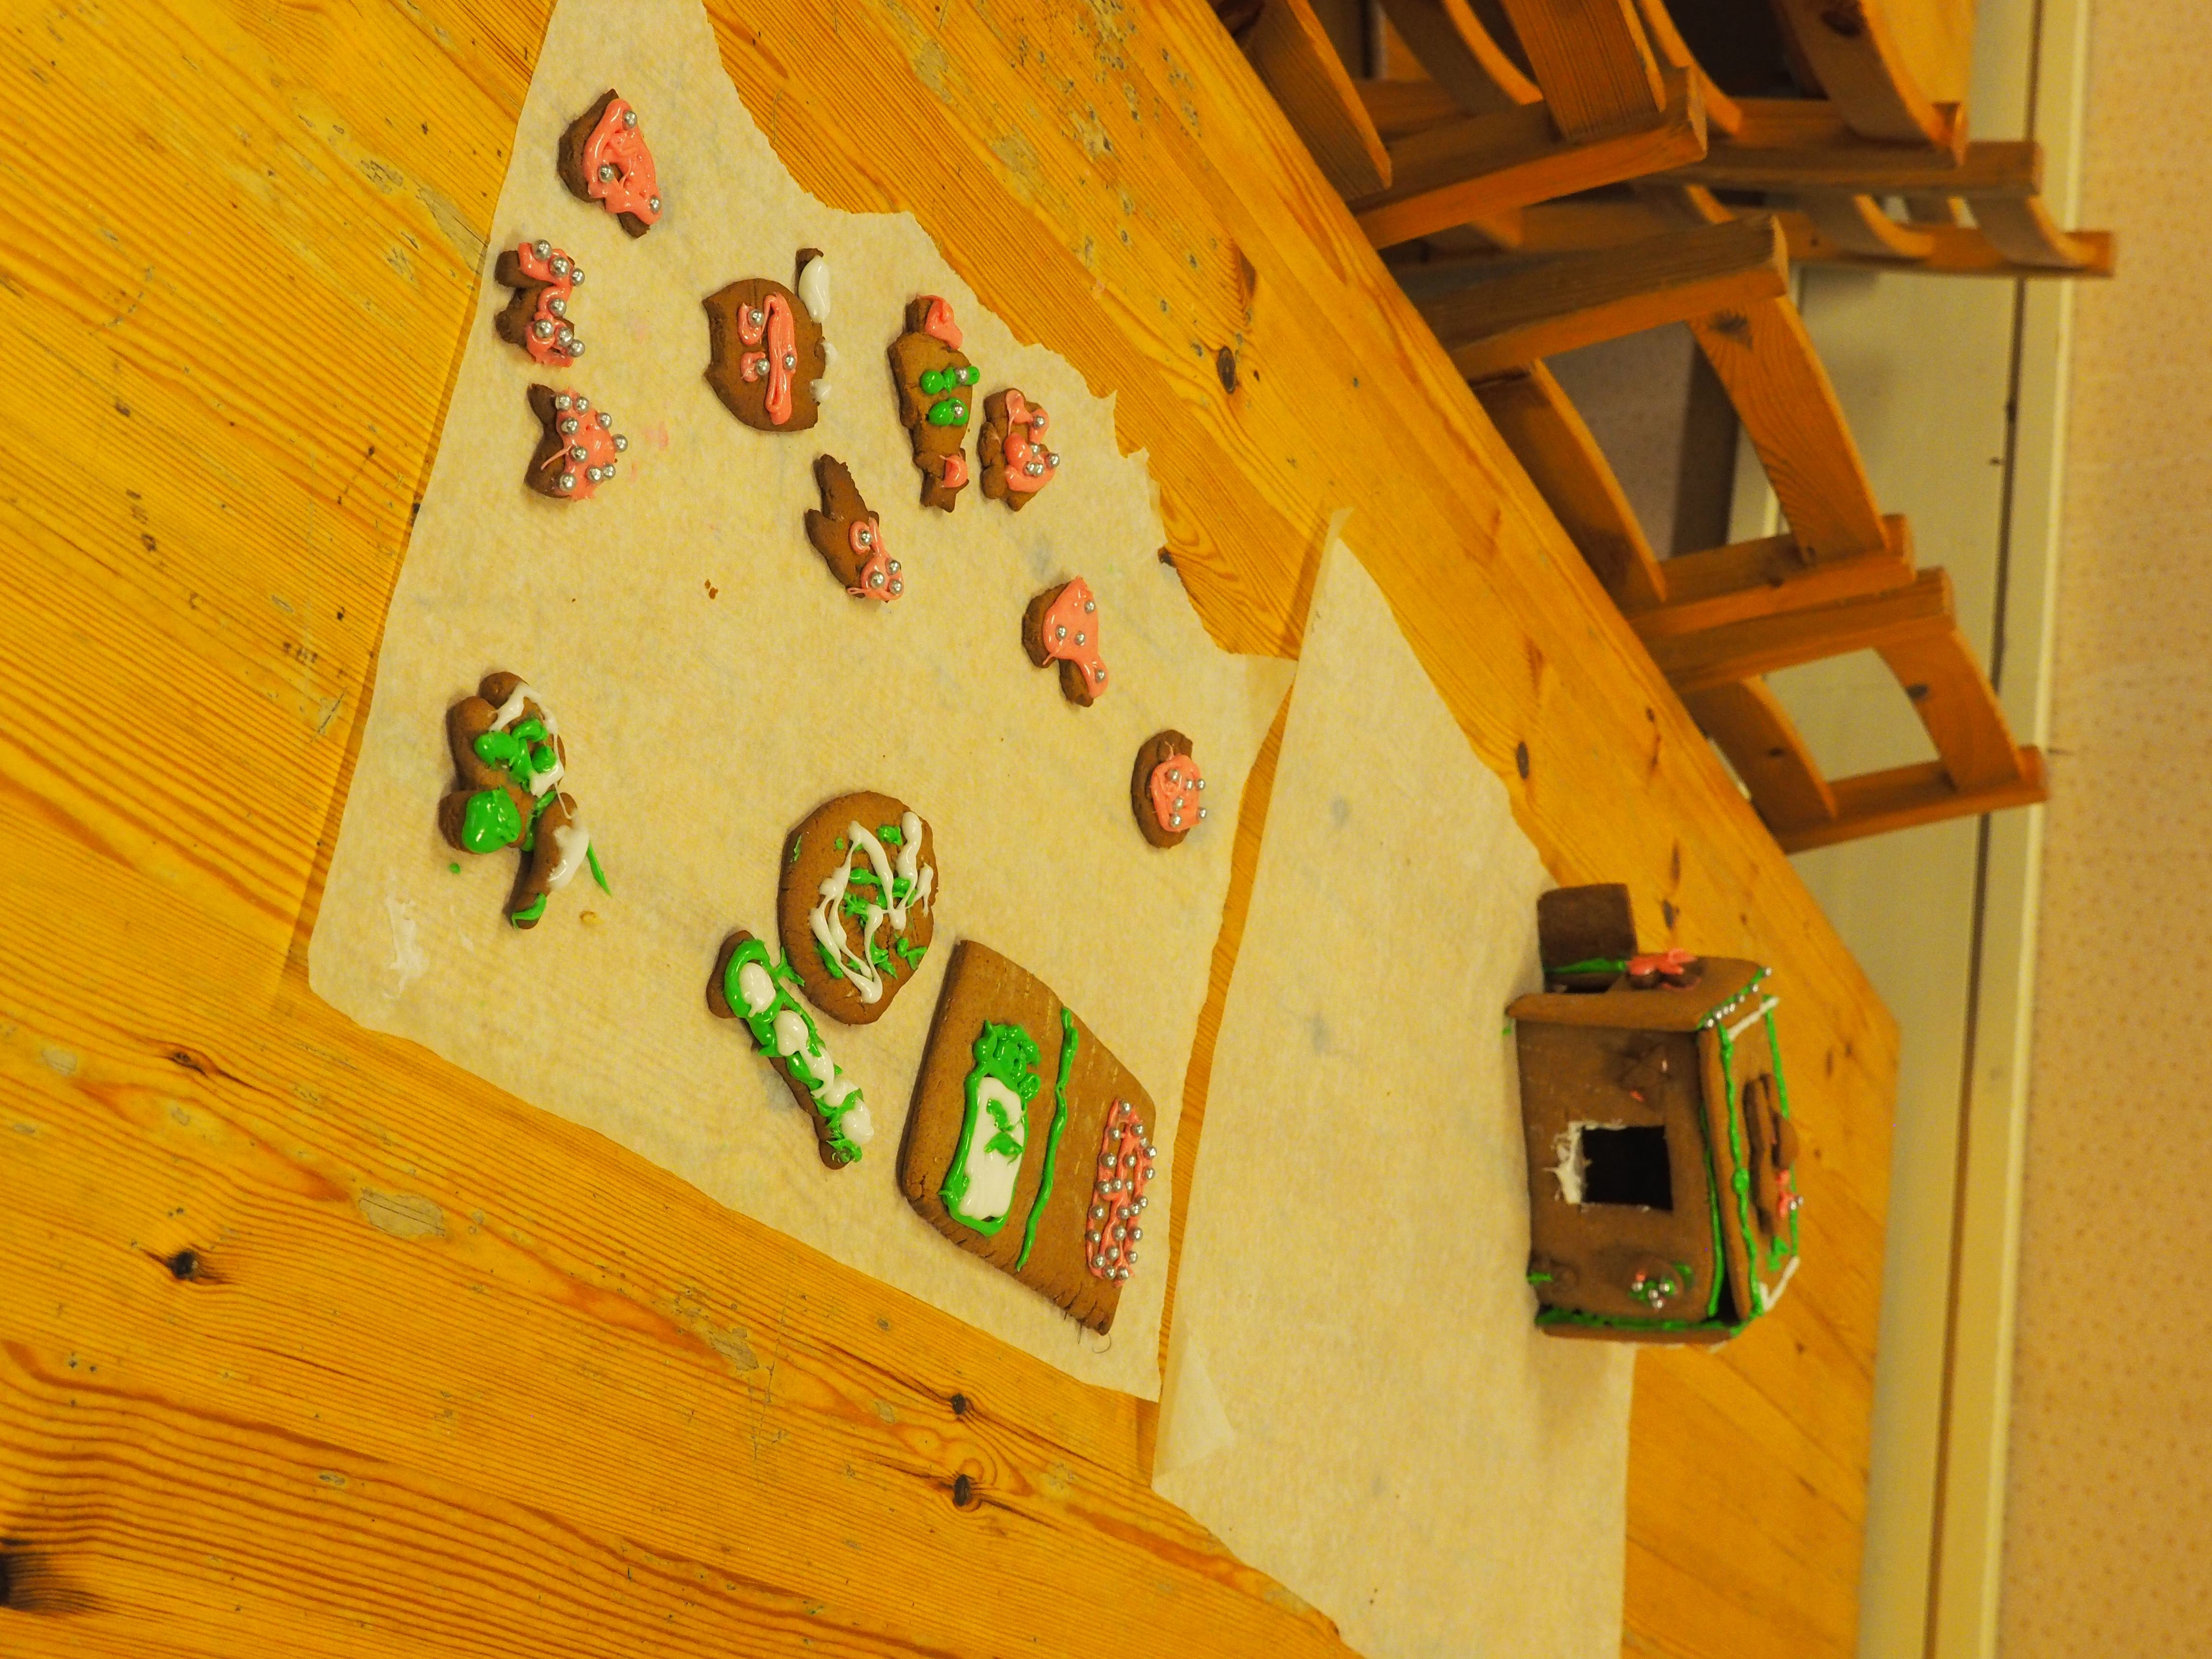
\includegraphics[width=.475\textwidth,height=.475\textwidth,keepaspectratio,angle=90]{assets/pipari2}

\vspace*{.05\textwidth}

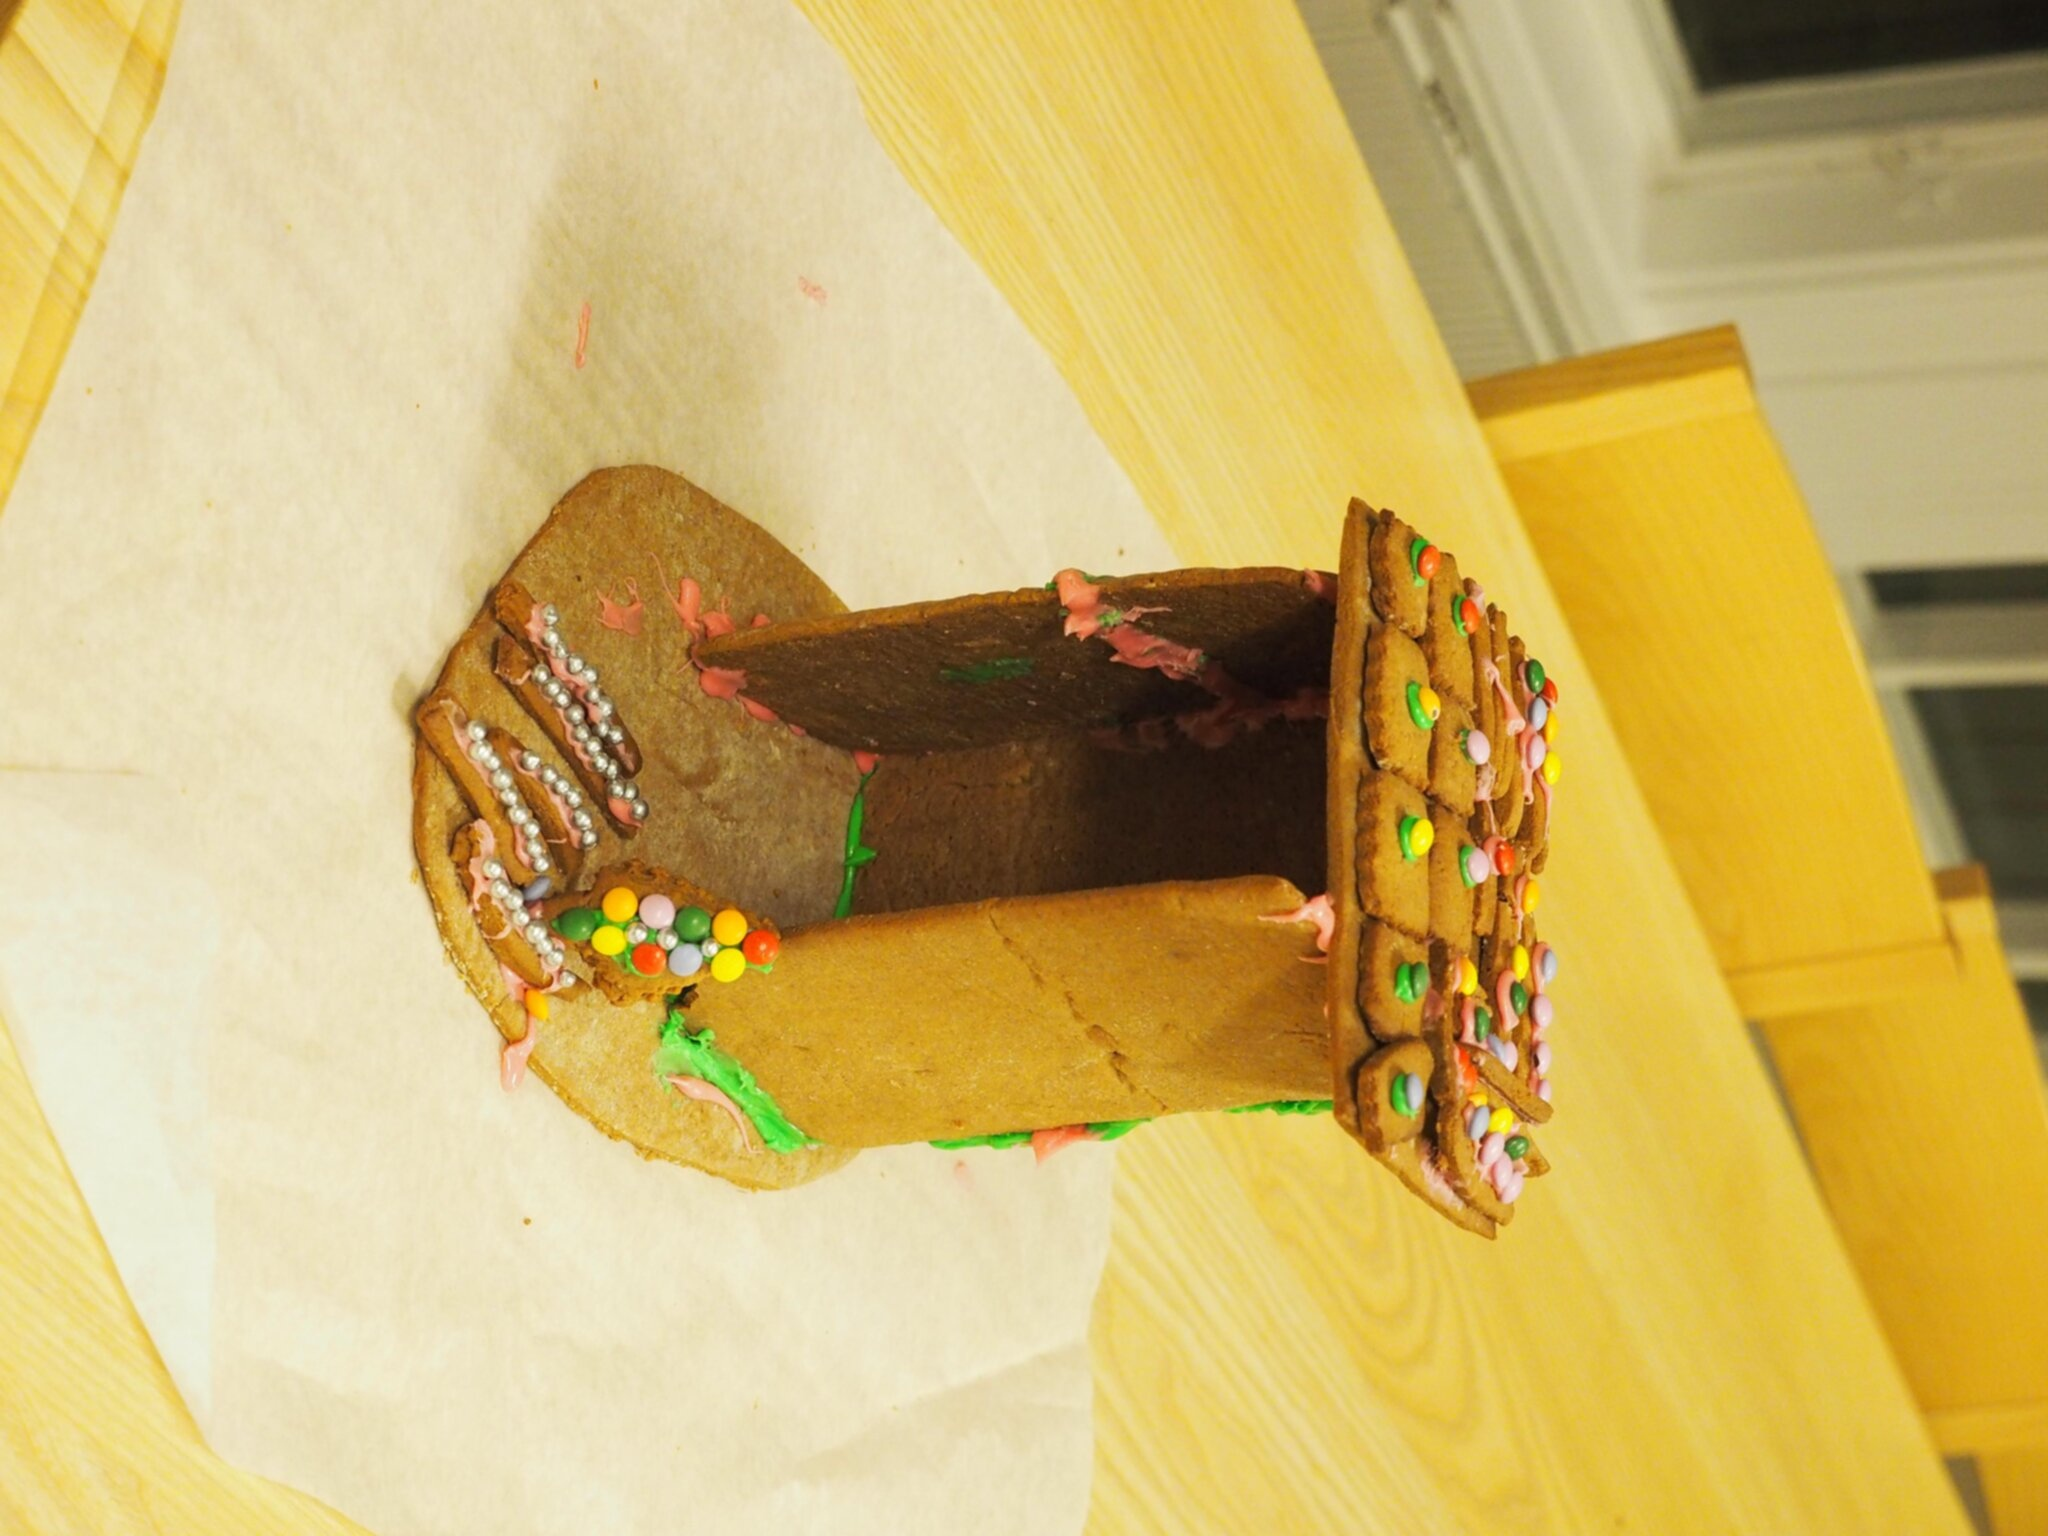
\includegraphics[width=.475\textwidth,height=.475\textwidth,keepaspectratio,angle=90]{assets/pipari4}\hfill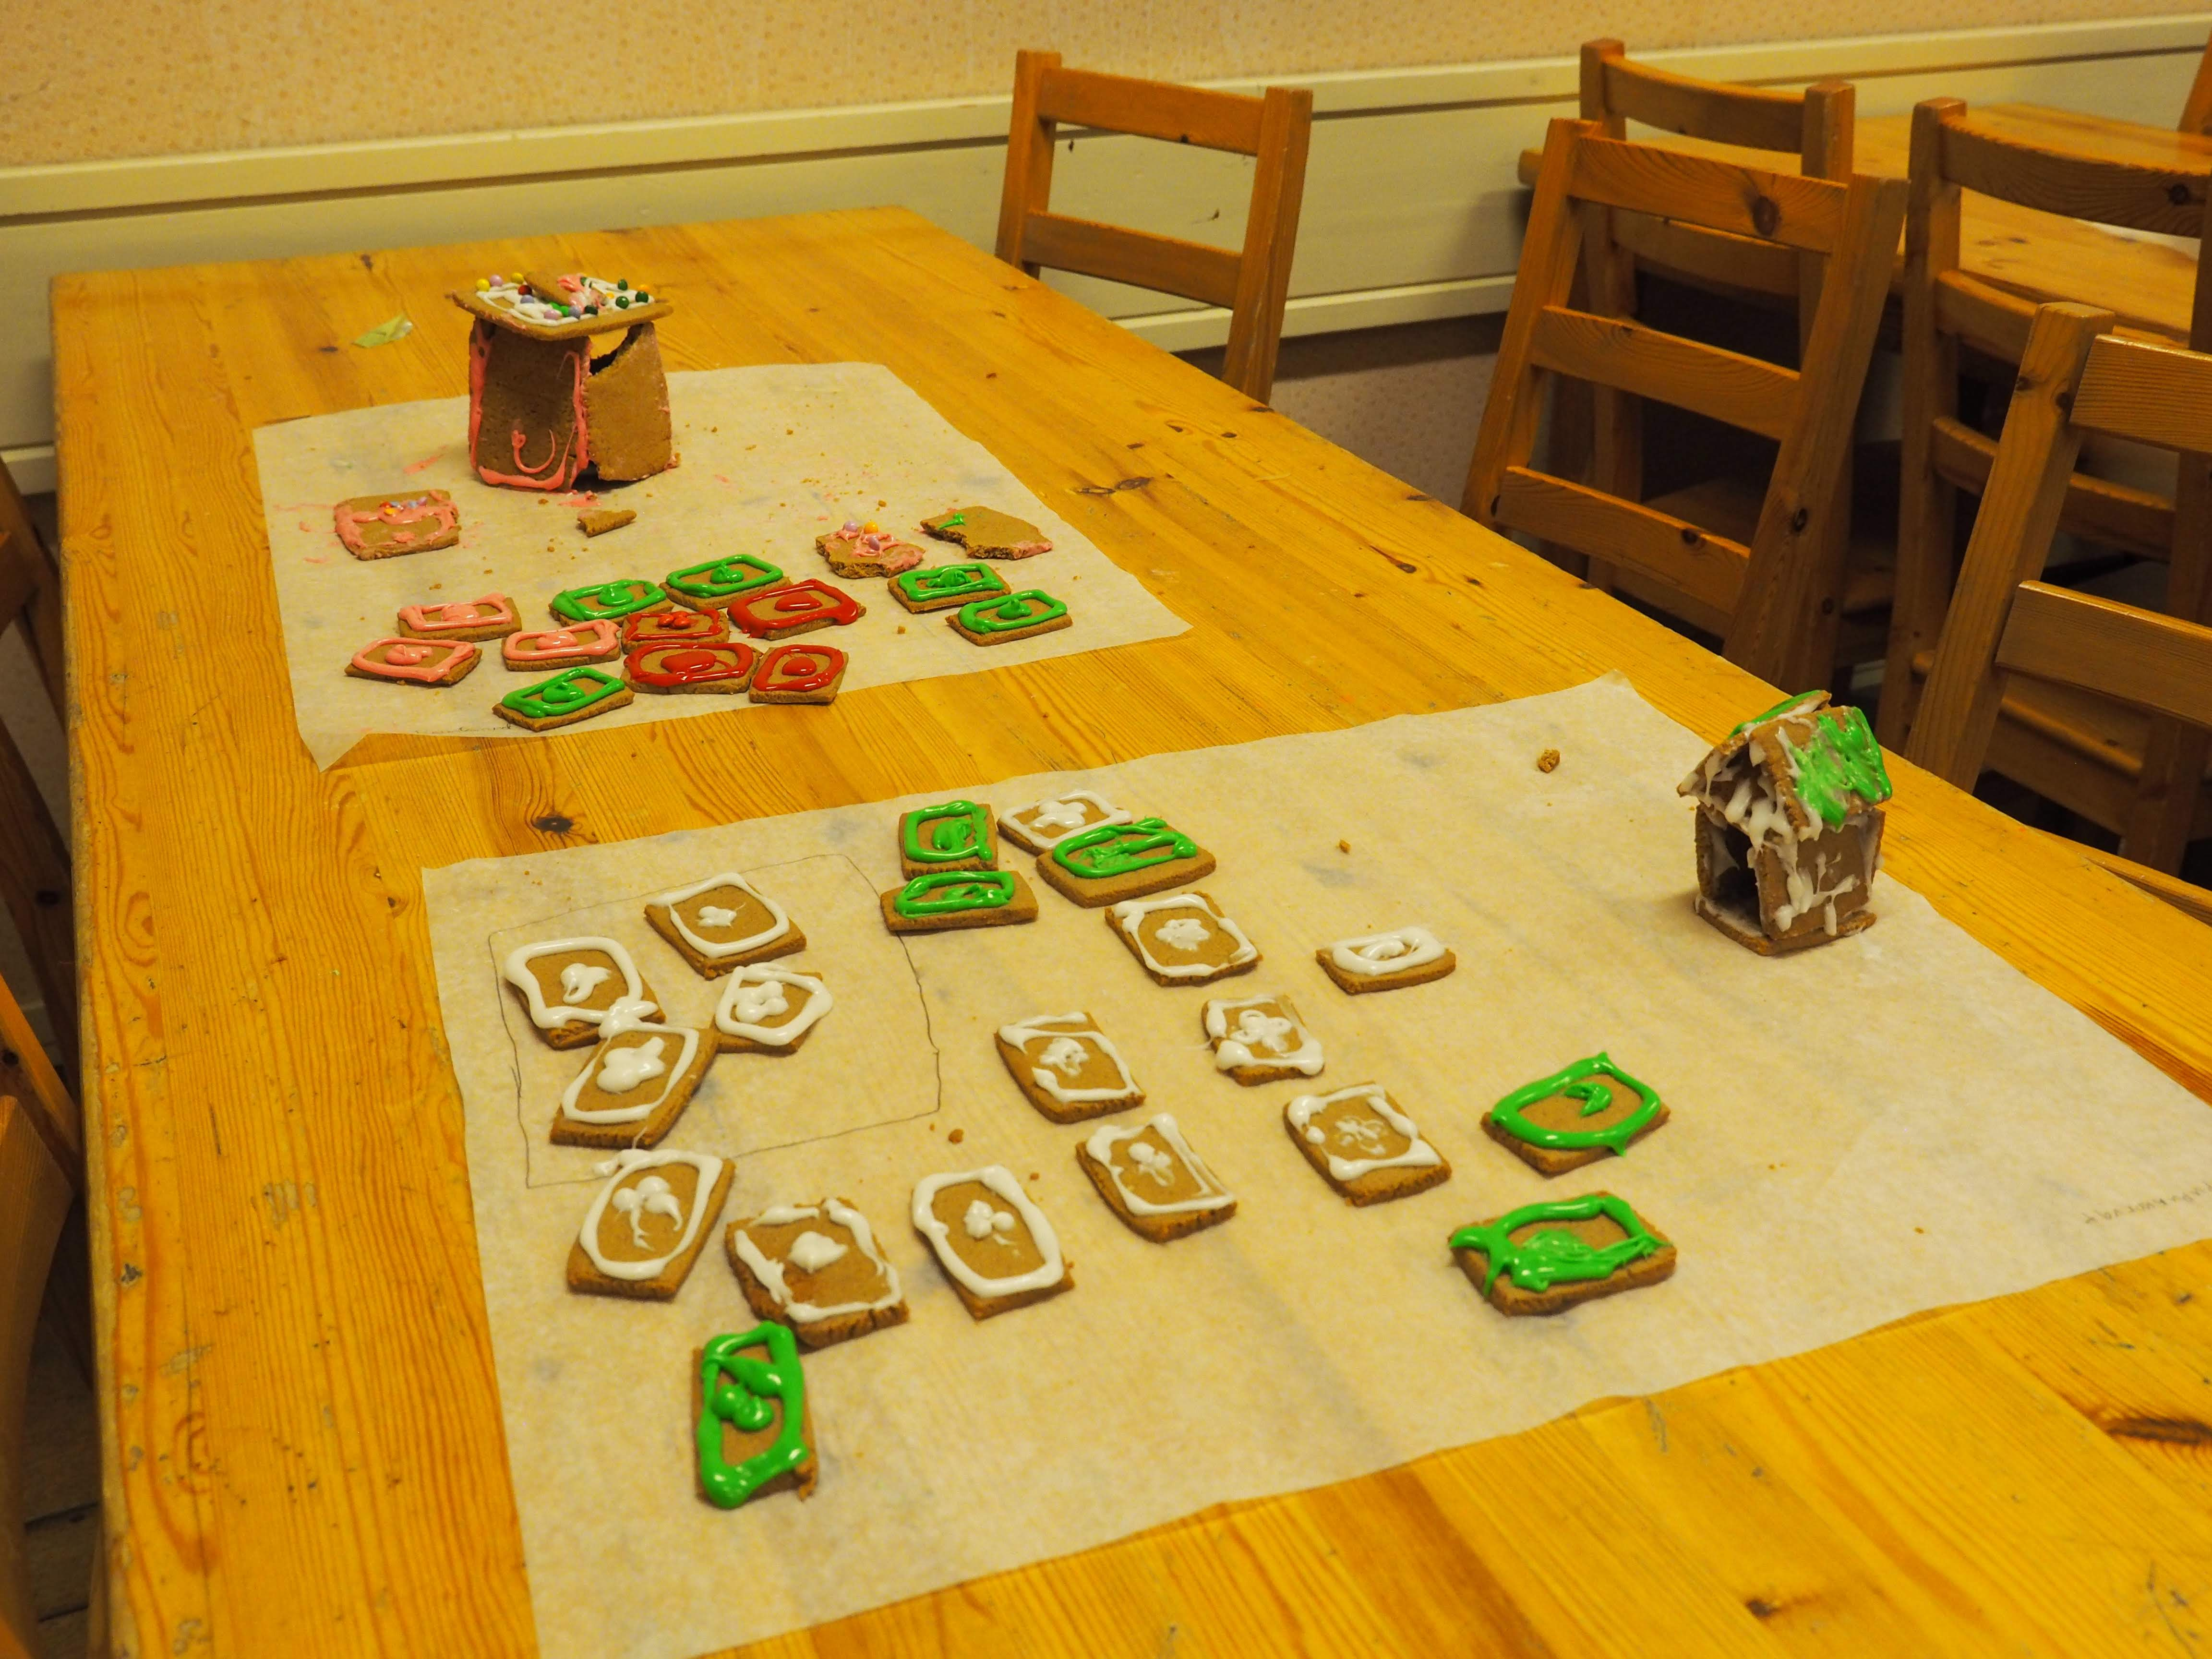
\includegraphics[width=.475\textwidth,height=.475\textwidth,keepaspectratio]{assets/pipari3}

\vspace*{.05\textwidth}

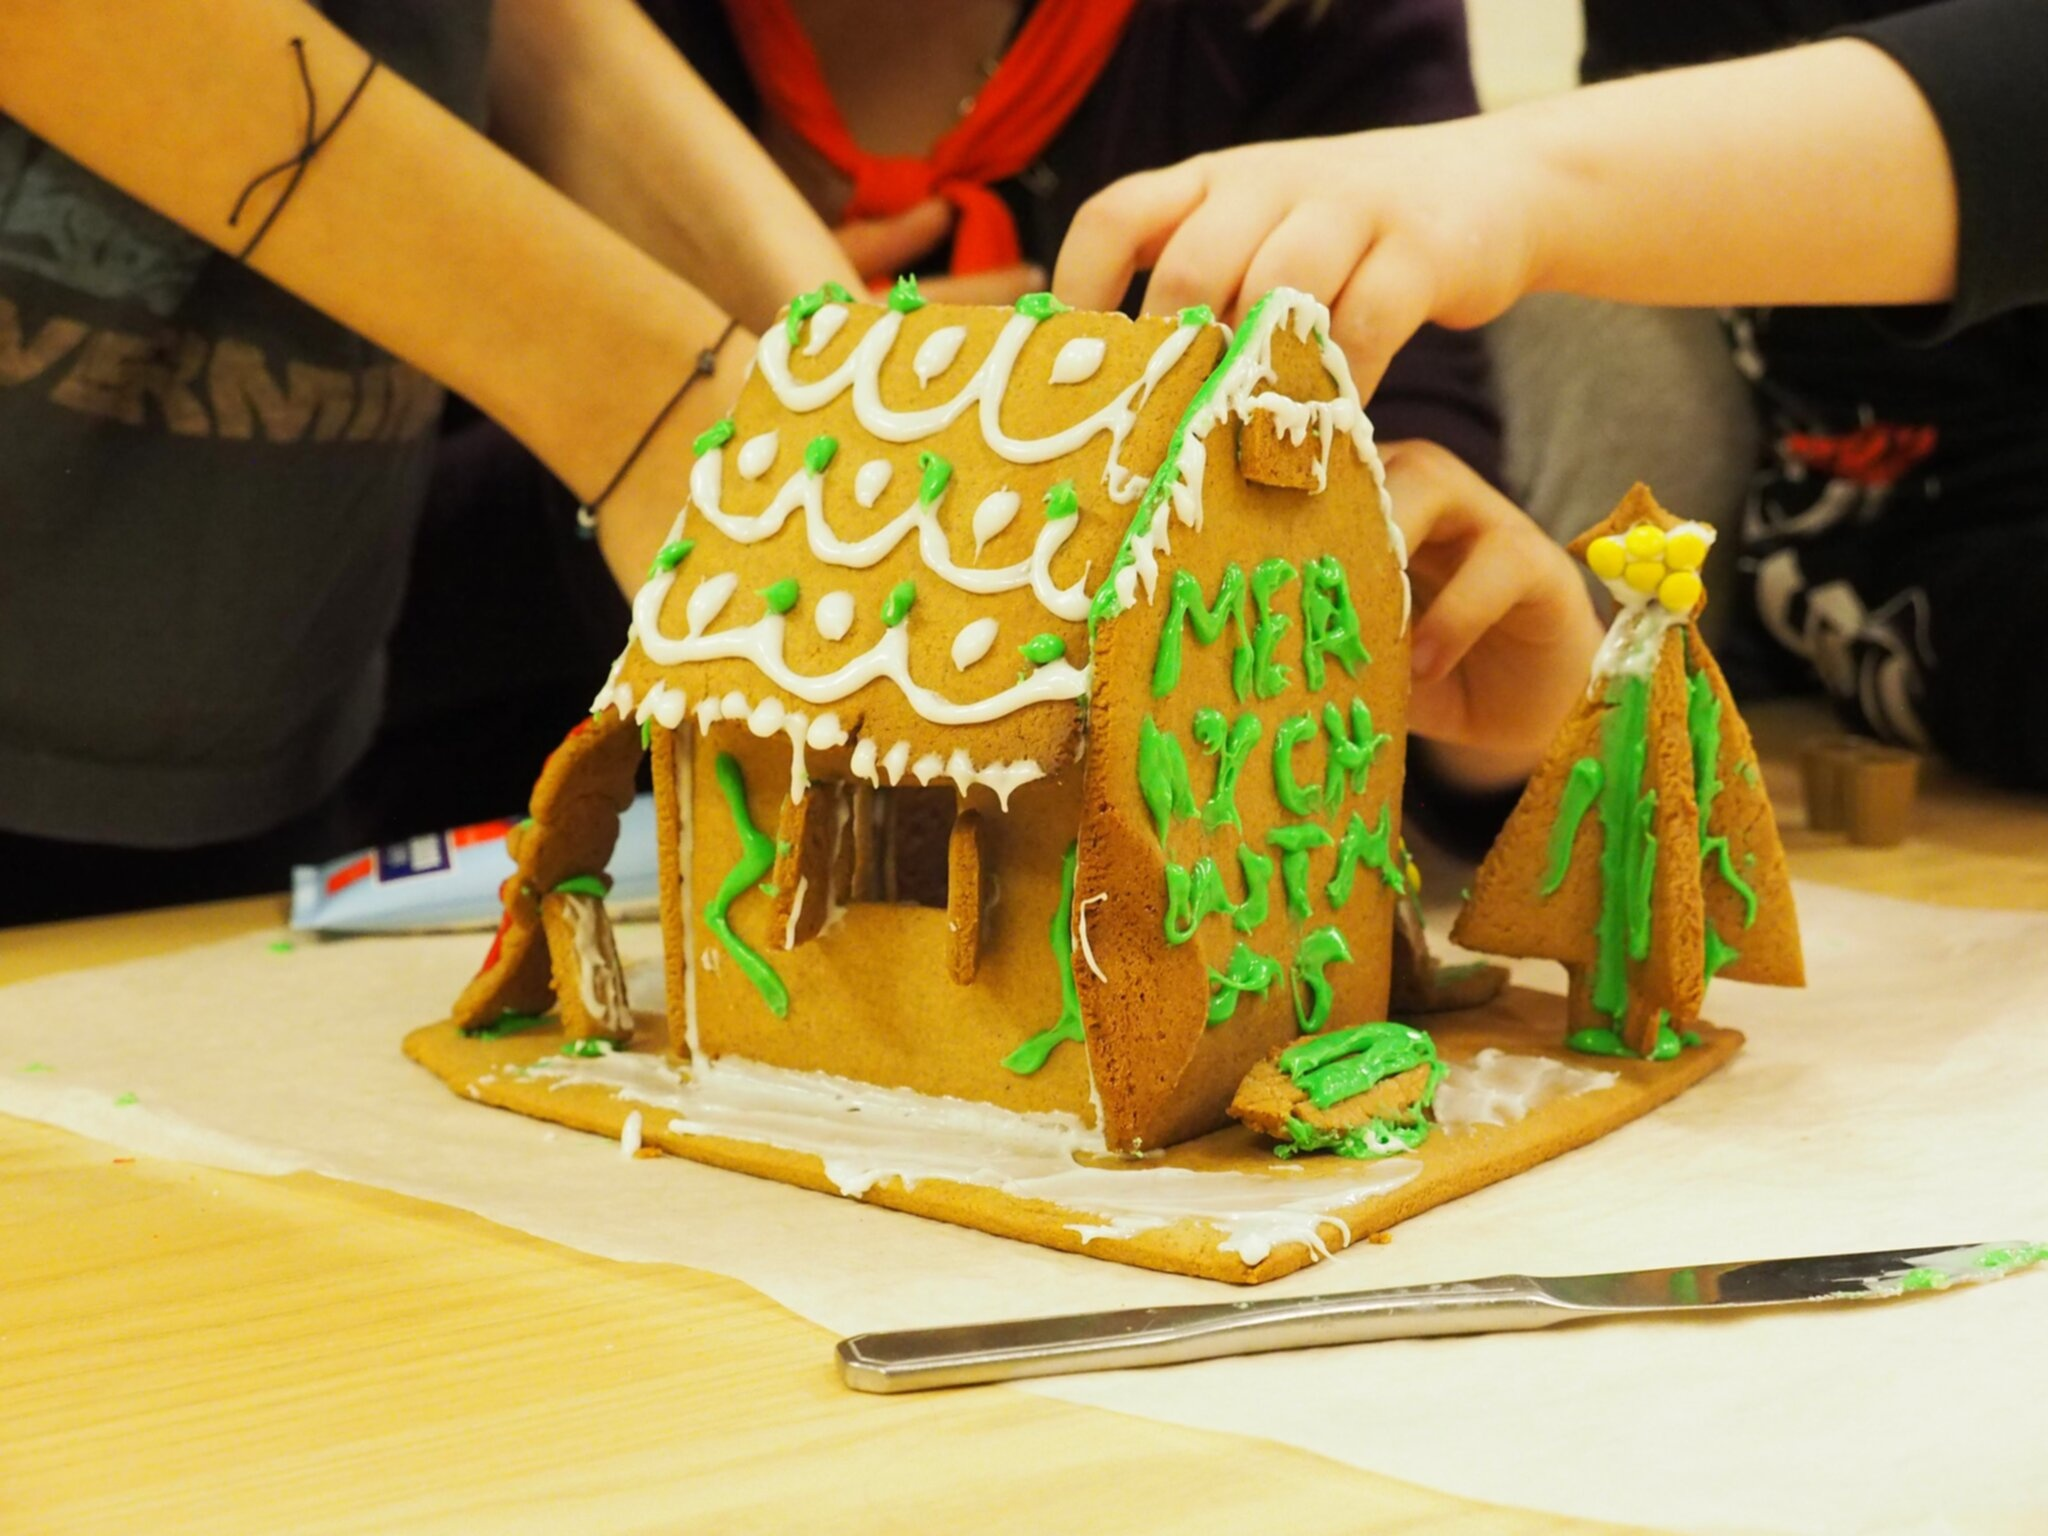
\includegraphics[width=.475\textwidth,height=.475\textwidth,keepaspectratio]{assets/pipari5}

\caption{Vartioiden piparkakkuteokset.}
\end{figure*}

Joulujuhlan juonsivat Tesla ja Touko ja se alkoi Päärynähyttysten 
spektaakkelimaisella näytelmällä joulupukista, tountuista ja nuuttipukista, 
joka huipentui joulupukin ja nuuttipukin eeppiseen räppäyskilpailuun! Listan 
joulujuhlassa ansioituneista löydät edellisestä Tassusta.

Juhlan päätyttyä luontotalo siivottiin loppuun ja lähdettiin kotimatkalle. 
Mitäköhän keksimmekään taas tämän vuoden pikkujouluretkelle?
\end{multicols}

\medskip

\noindent\null\hfill Kuvat: Janne ja Tanguy\\
\noindent\null\hfill Teksti: Janne
